%
% حق نشر 1390-1402 دانش پژوهان ققنوس
% حقوق این اثر محفوظ است.
% 
% استفاده مجدد از متن و یا نتایج این اثر در هر شکل غیر قانونی است مگر اینکه متن حق
% نشر بالا در ابتدای تمامی مستندهای و یا برنامه‌های به دست آمده از این اثر
% بازنویسی شود. این کار باید برای تمامی مستندها، متنهای تبلیغاتی برنامه‌های
% کاربردی و سایر مواردی که از این اثر به دست می‌آید مندرج شده و در قسمت تقدیر از
% صاحب این اثر نام برده شود.
% 
% نام گروه دانش پژوهان ققنوس ممکن است در محصولات دست آمده شده از این اثر درج
% نشود که در این حالت با مطالبی که در بالا اورده شده در تضاد نیست. برای اطلاع
% بیشتر در مورد حق نشر آدرس زیر مراجعه کنید:
% 
% http://dpq.co.ir/licence
%
% 
% در این بخش تمام توانایی‌های داگزی برای تولید نمودار در مستند نهایی مورد بحث قرار
% خواهد گرفت. این نمودارها با استفاده از ابزارها و تنظیم‌های متفاوتی ایجاد می‌شود
% که در اینجا هرکدام به صورت جداگانه مورد بررسی قرار گرفته است. ابزارهای مورد
% بررسی عبارت اند از
% 
% * mscgen
% * dot
% 
% \author maso
% \date تابستان ۱۳۹۱
% 
\chapter{گراف‌ها و نمودارها}

% FIXME: maso 1391: مقدمه‌ای بر گرافها و نمودارها اورده شود


یکی از بهترین روش های موجود در نشان دادن سلسله مراتب وراثتی در کد نویسی و بخصوص
در شی گرایی استفاده از گراف ها و نمودارهایی است که رابطه وراثت و کلاس ها را
نمایش می دهد.
با استفاده از گراف ها و نمودارها علاوه بر اینکه مستند یک ساختار مناسب بدست می آورد، خوانایی
کدهای نوشته شده نیز بهتر می شود. در نتیجه توسعه و بازبینی برنامه ها را افزایش می دهد.

\lr{doxygen}
 دارای ساختاری است که ازتولید دیاگرام های وراثت برای کلاس های \lr{C++}پشتیبانی می کند.
 \lr{doxygen}  برای تولید بیشتر گراف ها و نمودارهای پیشرفته
از\lr{graphviz}استفاده می کند.\lr{Grophviz} یک ابزار متن باز برای طراحی گراف و
شبیه سازی نمودار بر روی سکوهای مختلف است. ضمنا در آدرس:
 \href{http://www.graphviz.org/}{graphviz home} می توان به اطلاعات بیشتری دست پیدا کرد.
این ابزار دارای چند برنامه نمونه یا طرح اصلی است. در حالت
کلی شبیه سازی یک نمودار روشی است که توسط آن می توان اطلاعات ساختاری یک مجموعه
به هم مربوط را نمایش داد. بطور مثال نمایش نمودار انتزاعی از یک شبکه، نمایش یک
شبکه بیو انفورماتیک، روش های مهندسی نرم افزار، پایگاه داده، یادگیری ماشین و
...

\lr{Graphviz} تمام امکانات لازم برای طراحی نمودار هایی که نمونه های آن در بالا
ذکر شد را فراهم می کند. امکاناتی چون: واسط گرافیکی، ابزارهای کمکی، کتابخانه ها
و.... را برای آسان کردن پیاده سازی فراهم کرده است. 
بطور کلی این ابزار برای رسم گراف و نمودار تنها از یک زبان متنی ساده استفاده می کند.
\lr{Graphviz}
 دیاگرام خواسته شده را در شکل های گوناگون مانند تصاویر و  \lr{SVG} برای صفحات اینترنتی، \lr{pdf} یا \lr{postscript} برای الحاق به مستندهای دیگر و یا جهت نمایش در مرورگر نمودار تعاملی به نمایش در می آورد.
%در واقع این ابزار پیاده سازی هر گراف را با استفاده از یک زبان متنی ساده
%را فراهم کرده است که می توان با استفاده از این زبان و وارد کردن آن در مستند ها 
%\lr{doxygen} نمودار ها و گراف های مورد نظر را پیاده کرد.
 
البته علاوه بر
\lr{doxygen} می توان از این ابزار در تولید مستندها بصورت
\lr{XML} , \lr{GXL} و صفحات وب نیز استفاده کرد.
\lr{Graphviz} دارای ویژگی های مفید متعددی برای بهینه سازی و بهتر کردن نمودارها است. 
ویژگی هایی چون کنترل بر روی رنگ های یک نمودار، فونت، تغییر پوسته های یک جدول، تغییر پارامترهای یک خط، ابر پیوندها و ساخت شکل های خصوصی در این ابزار قابل دسترسی هستند.
\cite{graph}
حال اگرابزار\lr{"dot} را در دست داشته باشید، می توانید با نشاندن تگ 
\lr{HAVE-DOT}  به \lr{yes} در فایل پیکربندی، از آن در \lr{doxygen} استفاده کنید.\\
\lr{doxygen} برای تولید گرافهای زیر از ابزار \lr{"dot''} استفاده می کند.\\

%
% حق نشر 1390-1402 دانش پژوهان ققنوس
% حقوق این اثر محفوظ است.
% 
% استفاده مجدد از متن و یا نتایج این اثر در هر شکل غیر قانونی است مگر اینکه متن حق
% نشر بالا در ابتدای تمامی مستندهای و یا برنامه‌های به دست آمده از این اثر
% بازنویسی شود. این کار باید برای تمامی مستندها، متنهای تبلیغاتی برنامه‌های
% کاربردی و سایر مواردی که از این اثر به دست می‌آید مندرج شده و در قسمت تقدیر از
% صاحب این اثر نام برده شود.
% 
% نام گروه دانش پژوهان ققنوس ممکن است در محصولات دست آمده شده از این اثر درج
% نشود که در این حالت با مطالبی که در بالا اورده شده در تضاد نیست. برای اطلاع
% بیشتر در مورد حق نشر آدرس زیر مراجعه کنید:
% 
% http://dpq.co.ir/licence
%

\part{نمونه‌ها}

% در این پرونده تمام استاندارهای مورد نیاز برای نوشتن مستند در زبان برنامه سازی جاوا تعیین می‌شود
% این استاندارهای بر اساس رابطه میان javadoc و doxygen تعیین می‌شود.
\chapter{جاوا}
  زبان برنامه نویسی جاوا؟

%
% حق نشر 1390-1402 دانش پژوهان ققنوس
% حقوق این اثر محفوظ است.
% 
% استفاده مجدد از متن و یا نتایج این اثر در هر شکل غیر قانونی است مگر اینکه متن حق
% نشر بالا در ابتدای تمامی مستندهای و یا برنامه‌های به دست آمده از این اثر
% بازنویسی شود. این کار باید برای تمامی مستندها، متنهای تبلیغاتی برنامه‌های
% کاربردی و سایر مواردی که از این اثر به دست می‌آید مندرج شده و در قسمت تقدیر از
% صاحب این اثر نام برده شود.
% 
% نام گروه دانش پژوهان ققنوس ممکن است در محصولات دست آمده شده از این اثر درج
% نشود که در این حالت با مطالبی که در بالا اورده شده در تضاد نیست. برای اطلاع
% بیشتر در مورد حق نشر آدرس زیر مراجعه کنید:
% 
% http://dpq.co.ir/licence
%
% در این پرونده چگونگی نوشتن مستندهای سی بیان می‌شود. این استانداردهای بر اساس
% رابطه میان ابزارهای مستند نویسی با Doxygen تعیین خواهد شد.
% مصطفی برمشوری ۱۳۹۰
\chapter{استانداردهای زبان \lr{C/C++}}

در این فصل استانداردهایی برای مستندنویسی کدهایی که به زبان \lr{C/C++} نوشته
می‌شود شرح داده شده است. تمام مواردی که در فصل‌های قبل در مورد مستندنویسی گفته
شد همگی مورد قبول است. در این قسمت نحوه استفاده از این موارد در پروژه‌هایی که به
زبان \lr{C/C++}  نوشته شده‌اند را نشان می‌دهیم. در پروژه‌هایی به این زبان
پرونده‌های سرآیند و پیاده‌سازی وجود دارد که در این قسمت گفته می‌شود که در هر بخش
از پروژه چه مستندهایی نوشته می‌شود.

\section{مستند فنی}
% FIXME : مصطفی ۱۳۹۰-۱۲ :  
% مستند فنی در پرونده‌های سرآیند نوشته می‌شود.
% تمام برچسب‌ها بر اساس استاندار Qt است تا همه را پوشش دهد

در زبان برنامه سازی سی، پرونده‌های سرآیند تنها پرونده‌هایی هستند که بدون ترجمه
انتقال داده می‌شوند. این پرونده‌ها تعیین می‌کند که در پرونده‌های باینری ایجاد
شده چه توابع و موجودیت‌هایی وجود دارد و لینکر چگونه باید پیوندهای مورد نیاز را
ایجاد کند. از آنجا که این پرونده‌ها همواره به عنوان جزئی از خروجی انتقال داده
می‌شوند بهتر است که مستندهای فنی در این پرونده‌ها نوشته شود.

نوشتن مستندهای فنی در پرونده‌های سرآیند منجر به افزایش حجم داده در زمان انتقال
محصول می‌شود. فرض کنید که پروژه‌ای ایجاد شده است، در این صورت در فرآیند انتقال
نیاز است علاوه بر محصول مستندهای تکنیکی نیز به نحوی همراه با محصول انتقال داده
شود، در این صورت مستند فنی علاوه نه تنها به صورت مستقل بلکه همراه با پرونده‌های
سرآیند وجود دارد.

گرچه درنگاه اول افزایش حجم محصول یک ایراد اساسی برای نوشتن مستندهای فنی در
پرونده‌های سرآیند به شمار می‌آید اما با این حال از دیدگاه پیاده ساز به عنوان یک
مزیت در نظر گرفته می‌شود. توسعه دهندگان یک سیستم بدون نیاز به مراجعه به کد
برنامه می‌توانند به مستند فنی آن دست پیدا کنند. بسیاری از محیط‌های مجتمع توسعه
(مانند \lr{Eclipse}) مستندهای نوشته شده در پرونده‌های سرآیند را به عنوان مستند
یک موجودیت برای کاربران نمایش می‌دهد. علاوه بر این می‌توان با استفاده از ابزارهای
مناسب پیش از ایجاد یک محصول، مستندهای فنی موجود در پرونده‌های سرآیند را از محصول
حذف کرد.

\begin{note}
گرچه تنها مستند موجود در پرونده‌های سرآیند، مستند فنی است و توسعه دهندگان سیستم
باید از نوشتن مستند پیاده سازی در این پرونده‌ها خودداری کنند، اما در صورت لزوم
می‌توان برخی از مستندهای پیاده سازی را نیز در پرونده‌های سرآیند نوشت.
\end{note}

زبان برنامه‌سازی \lr{C/C++} یک زبان مترجمی است از این رو بدیهی است که برخلاف
زبانهای قابل حملی مانند \lr{java} قابلیت ترجمه و اجرا برای تمام محیط‌های
نرم‌افزاری و سخت افزاری را نداشته باشد. بدیهی است که در چنین شرایطی مستند فنی
باید به صورت جزئی تمام پیشنیازهای محصول را تعیین کند. برای نمونه فرض کنید که
محصول مورد نظر یک بسته ریاضی است که از دستورالعمل‌های خاصی برای انجام پردازش‌های
خود استفاده می‌کند، در این صورت مستند فنی باید به صورت کامل پردازنده‌های مورد
حمایت را معرفی و نتیجه استفاده از پردازنده‌های دیگر را به صورت کامل تشریح کرده
باشد.

همانگونه که پیش از این نیز اشاره شده، ابزارهای متفاوتی برای ایجاد مستند فنی بر
اساس کد تولید شده در بازار موجود می‌باشد. برای نمونه ابزارهایی مانند \lr{QtDoc}
و \lr{CDoc} دو نمونه از ابزارهایی است که برای ایجاد مستند فنی از پروژه‌هایی که
به زبان برنامه سازی \lr{C/C++} ایجاد شده اند، مورد استفاده قرار می‌گیرند. از این
رو مستند‌های فنی باید به گونه‌ای نوشته شود که بتوان با استفاده از ابزارهای دیگر
نیز مستند فنی مناسبی را ایجاد کرد. برای نمونه در مستندگر \lr{QtDoc} برچسب‌ها را
با استفاده از \textbackslash آغاز می‌شود، از این رو نوشتن تمام برچسب‌ها با استفاده
از این نمادگزاری قابلیت استفاده از این مستندگر را نیز فراهم می‌کند.
علاوه بر این در این مستندگر، برچسب‌های تعریف نشده نادیده گرفته می‌شود از سویی
تمام برچسب‌های تعریف شده در آن، در \lr{Doxygen} نیز تعریف شده است. از این رو
استفاده از تمام برچسب‌های تعریف شده در \lr{Doxygen} برای توسعه مستند فنی بسیار
مناسب است.

مستند فنی هر موجودیت ، در پرونده‌های سرآیند و پیش از آن موجودیت ایجاد می‌شود. در
این مستند باید توضیحات مناسب برای آن موجودیت ایجاد شده و پیوندهای مورد نیاز به
مستندهای وابسته نیز ایجاد شود.

برای نمونه یک کلاس را به عنوان موجودیت در نظر بگیرید، در این صورت علاوه بر
توضیحات کلی در مورد کاربرد و نحوه استفاده از این کلاس، باید اطلاعات دیگری در
مورد نویسنده، تاریخ ایجاد، و نسخه‌هایی که کلاس در آنها ایجاد شده است، به صورت
کامل تشریح شده باشد. برای نمونه کد زیر را در نظر بگیرید:

\begin{latin}
\lstset{language=C++}  
\begin{lstlisting}[frame=single] 
/**
 * \brief <Brief information>
 * 
 * <Detail information>
 * 
 * \see <Other document>
 * \since <First version>
 * \data <Creation Date>
 * \author <Author name>
 */
 class ClassName: public Parent{
 ...
 }
\end{lstlisting}
\end{latin}

همان گونه که در این نمونه مستند قابل مشاهده است، ابتدا به صورت خلاصه در مورد
کلاس نوشته شده و در ادامه به صورت کامل کاربردها و روش‌های استفاده از آن تشریح
شده است. در انتهای مستند اطلاعات جامعی از مستند‌های وابسته، نسخه و
تاریخ ایجاد، و توسعه دهنده آن به صورت کامل آورده شده است. برای نمونه در مستند
زیر تمام اطلاعات مورد نیاز برای یک تابع نوشته شده است:

\begin{latin}
\lstset{language=C++}  
\begin{lstlisting}[frame=single] 
/**
 * \brief <Brief information>
 * 
 * <Detail information>
 * 
 * \see <Other document>
 * \since <First version>
 * \param <param name> <param information>
 * \return <return information>
 */
QString toString(int base, ...);
\end{lstlisting}
\end{latin}

همانگونه که در نمونه بالا قابل مشاهده است ابتدا یک توصیف کوتاه و سپس توصیف کامل
از تابع آورده شده است. در انتهای مستند نیز اطلاعات مورد نیاز در مورد مستندهای
مرتبط، نسخه ایجاد، پارامترهای و خروجی تابع تشریح شده است.

\begin{note}
در پروژه‌هایی که به زبان برنامه نویسی \lr{C} نوشته می‌شود، اطلاعات مشابه در
ابتدایی پرونده سرآیند آورده می شود.
\end{note}

یکی دیگر از موجودیت‌های مهم در پروژه‌های \lr{C/C++} توابع هستند. توابع به عنوان
جعبه‌هایی اجرایی در نظر گرفته می‌شوند که ورودی‌ها را به خروجی تبدیل می‌کنند. در
اینجا نیز علاوه بر توضیحات کلی باید مواردی مانند، پارامترهای ورودی خروجی،
استثناها، نسخه‌ ایجاد شده و مستندهای وابسته نیز در مستند آورده شده باشد.


\section{مستند پیاده‌سازی}
% FIXME : مصطفی ۱۳۹۰-۱۲ : روش نوشتن مستند فنی
% مستند فنی در پرونده‌های cpp نوشته می‌شود و نباید در پرونده‌های سرآیند اورده شود.
% این مستندها ساختار خاصی نداشته و باید از اصول ابتدایی پیروی کنند

مستندات پیاده‌سازی را فقط و فقط باید در پرونده‌های پیاده‌سازی، یعنی پرونده‌های
\lr{.c} یا \lr{.cpp} نوشته شود. هرگز نباید در مورد نحوه پیاده‌سازی یا مواردی از
این دست در پرونده‌های سرآیند مطلبی قرار داده شود.
از آنجا که مستندات پیاده‌سازی برای توسعه‌دهندگانی است که قصد توسعه یا ادامه
پروژه را دارند بهتر است مستندات به گونه‌ای باشد که کار را برای درک کد ساده‌تر
کند. مثلا نیاز نیست برای قسمت‌های ساده مستند نوشت.
معمولا مستندات پیاده‌سازی را باید برای قسمت‌های پیچیده کد نوشت و یا هنگامی که
بخواهیم نکته‌ای را به توسعه‌دهندگان بعدی گوشزد کنیم. بنابراین نباید بی جهت کد را
شلوغ کرد.

پیمان‌نامه\footnote{\lr{Lincense}}  نوعی مستند پیاده‌سازی است یا بهتر بگوییم
مطالبی است که جز مستندات پیاده‌سازی محسوب می‌شود. یک پروژه یا نرم‌افزار ممکن است
پیاده‌سازی‌های مختلفی داشته باشد و هر یک پیمان‌نامه متفاوتی داشته باشد به همین
دلیل باید پیمان‌نامه در مستندات پیاده‌سازی ذکر شود. اگر در یک پیاده‌سازی خاص،
قسمت‌هایی باشند که پیمان‌نامه متفاوتی از دیگر قسمت‌ها دارد باید دقیقا قبل از
قسمت‌ها پیمان‌نامه مربوط به آن آورده شود.

یکی از موارد مهمی که باید در مستندات پیاده‌سازی آورده شود مشخصات سیستمی است.
مستندات سیستمی از جمله مواردی است که هم در مستند فنی می‌آید و هم در مستند
پیاده‌سازی با این تفاوت که در مستند پیاده‌سازی به صورت جزیی‌تر مثلا با ذکر دلیل
نوشته می‌شود. به عنوان مثال فرض کنید تمام یا قسمتی از یک تابع برای سیستم‌عامل
خاصی نوشته شده باشد و یا اینکه تنها روی پردازنده خاصی کار کند آنگاه در مستند
پیاده‌سازی می‌توان ضمن ذکر این موضوع علت آن را هم بیان کرد. مثلا می‌توان در
مستند پیاده‌سازی تابع مورد نظر نوشت: ``این تابع برای پردازنده‌های \lr{Intell}
مدل \lr{Core i7 AVX} به بعد پیاده‌سازی شده است چون در این تابع از مجموعه
دستورالعمل‌های \lr{AVX} استفاده شده است. به همین دلیل این تابع مخصوص
پردازنده‌هایی است که از این مجموعه دستورالعمل‌ها حمایت می‌کنند.''

مستند پیاده‌سازی مکان خاصی برای نوشتن ندارد ولی بهتر است مطالب مربوط به هر قسمت،
موجودیت، قطعه کد و ... قبل از آن بیاید. با استفاده از برچسب‌ها (برچسب‌هایی مثل
\lr{FIXME}، \lr{TODO}، \lr{WARNING} و ...) می‌توان درجه اهمیت مطالب را مشخص کرد.

در یک کار گروه موردی که بسیار به چشم می‌خورد این است که ممکن است بخش‌هایی از
پیاده‌سازی پروژه در مقاطع زمانی مختلف توسط افراد مختلف توسعه، بهبود یا بازنویسی
شود. در این موارد نکته‌ای که باید رعایت کرد این است که مستندات پیاده‌سازی نوشته
شده توسط نویسنده‌های قبلی را نباید حذف کرد. در صورتی که کد ویرایش می‌شود و نیازی
به نوشتن مستند پیاده‌سازی است قبلی مستند جدید به همراه نام نویسنده جدید و تاریخ
ویرایش آن پایین مستند قبلی نوشته شود.
مستندات نویسندگان قبلی در صورتی حذف می‌شوند که قسمت‌های پیاده‌سازی‌ای که آن
مستندات مربوط به آن‌ها هستند به طور کامل از پروژه حذف شوند.



\section{ساختار پروژه}

ساختار کلی پروژه‌های \lr{C/C++} نیز در حالت کلی بر اساس همان ساختاری است که در
گفتار پیش به آن اشاره شده است. اما بر اساس توانایی‌ها و اصول مطرح در زبان این
زبان برنامه سازی مبایست برخی تغییرها را در ساختار کلید لحاظ کرد. در این بخش
تغییرهای مورد نیاز در ساختار کلی پروژه به صورت کلی بررسی خواهد شد.

همانگونه که گفته شده تمام مستندهایی که به صورت مستقیم در رابطه با کد سیستم ایجاد
شده نیست، در یک پوشه جداگانه به نام \lr{doc} ایجاد می‌شود. تمام این مستندها با
پسوند \lr{*.doxy} بوده و حاوی اطلاعات جامعی در مورد مبانی، پیش نیازها، روشهای
نصب و دیگر موارد خواهد بود.

تمام برنامه‌های نوشته شده، مانند پرونده‌های سرآیند و پیاده سازی‌ها در پوشه
\lr{src} قرار می گیرد.
توابع و کلاس‌های تعریف شده در پروژه باید به صورت منطقی (و یا بر اساس فضاهای
تعریف شده در پروژه) در پرونده‌های سرآیند تعریف شده و به صورت مستقیم در مسیر
\lr{src} قرار بگیرد. معادل با هر پرونده سرایند و یا بر اساس منطق سیستم،
پوشه‌هایی ایجاد شده و پیاده سازی تمام توابع و کلاس ها در پرونده‌هایی با پسوند
\lr{*.cpp, *.c, *.cuda}در این پوشه‌ها ایجاد می‌شود.

\begin{figure}
	\centering
    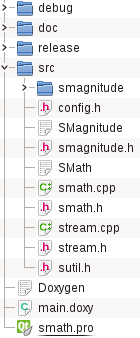
\includegraphics[width=0.25\textwidth]{image/standards-cpp-project-struct}
    \caption[ساختار مورد نیاز برای ایجاد مستند تکنیکی در پروژه‌های \lr{C/C++}]
    {
      
    }
    \label{standards-cpp-struction}
\end{figure}

برنامه‌های زبان برنامه سازی \lr{C/C++} را می‌توان با استفاده از روش‌های متفاوتی
ترجمه کرد. یک روش ترجمه زمانی است که پروژه به صورت کامل تست شده و آماده فاز
تحویل پروژه‌ است. در این فاز با استفاده از برنامه‌های بهینه ساز یک ترجمه بهینه
از پروژه ایجاد می‌شود که به مراتب سریع‌تر از حالت عادی پروژه است. از این رو یک
پوشه به نام  \lr{release} در پروژه ایجاد شده و همواره نتیجه ترجمه نهایی پروژه در
آن ایجاد می‌شود.

ترجمه دیگری که در طی فرآیند توسعه سیستم مورد استفاده قرار می‌گیرد، حالت اشکال
زدا است. در این حالت کدهای اضافه به صورت خودکار به پروزه اضافه شده تا برای دنبال
کردن خط به خط پروژه مناسب باشد. نتایج به دست آمده از این ترجمه نیز در مسیری به
نام \lr{debug} ایجاد می شود.

در نهایت می‌توان با استفاده از ابزارهای مناسب و بر اساس این ساختار، به صورت
خودکار محصول نهایی همراه با مستند تکنیکی را ایحاد کرد. اما پیش از هر چیز نیاز
است که فهرست کاملی از پرونده‌های سرآیند و برنامه‌های نوشته شده ایجاد شود تا
ابزارها بتوانند سرآیندها و برنامه‌های مورد نیاز برای نصب را تعیین کنند. برای
تعیین این پرونده‌ها یک پرونده به نام \lr{<project name>.pro} ایجاد می شود و در
آن فهرست کامل پرونده‌ها ایجاد می‌شود.

\begin{note}
نام این پرونده باید هم نام با پروژه باشد. به یاد داشته باشید که پروژه باید به
صورت کامل در یک پوشه به نام پروژه ایجاد شده باشد، برای نمونه در شکل
\ref{standards-cpp-struction} نه تنها نام پرونده \lr{*.pro} بلکه نام پوشه اصلی
پروژه، هم نام با خود پروژه است.
\end{note}

نام تمام پرونده‌ها با استفاده از کلمه کلید \lr{HEADERS} تعیین می‌شود، در حالت
کلی تعیین پرونده‌های سرآیند به صورت زیر است:

\begin{latin}
\lstset{language=C++}  
\begin{lstlisting}[frame=single] 
HEADERS += <header name> \ 
	... \
	<header name>
\end{lstlisting}
\end{latin}

پرونده‌های پیاده سازی نیز با استفاده از کلمه کلیدی \lr{SOURSES} تعیین می‌شوند.
در حالت کلی این فهرست به صورت زیر ایجاد خواهد شد.

\begin{latin}
\lstset{language=C++}  
\begin{lstlisting}[frame=single] 
SOURCES += <source name> \ 
	... \
	<source name>
\end{lstlisting}
\end{latin}

گاهی ممکن است که پرونده‌های سرآیند و کدهای ایجاد شده تنها برای یک سیستم‌عامل خاص
باشد، در این صورت باید به صورت کامل و تفکیک شده تعیین شوند. در نمونه زیر بر اساس
سکویهای متفاوت کدها و پرونده‌های سرآیند تفکیک شده اند:

\begin{latin}
\lstset{language=C++}  
\begin{lstlisting}[frame=single] 
HEADERS += src/test.h

CONFIG(win) { 
    SOURCES += src/test/win_imp1.cpp \
	src/test/win_imp2.cpp
}
CONFIG(unix) { 
    SOURCES += src/test/unix_imp1.cpp \
	src/test/unix_imp2.cpp
}
\end{lstlisting}
\end{latin}

در این نمونه فرض شده است که برای پرونده سرآیند \lr{test.h} دو نوع پیاده سازی
برای سیستم‌عاملهای یونیکس و ویندوز وجود دارد. از این رو در هر سکو باید
پرونده‌های مناسب ان در محصول نهایی قرار گیرد.
    

\subsection{ساختار پرونده \lr{*.h}}
در یک پرونده سرآیند معمولا تعاریف کلاس‌ها، متدها، توابع و ... آورده می‌شود و
علاوه بر این‌ها باید مستندات این موجودیت‌ها نیز در پرونده‌های سرآیند آورده شود.
ساختاری که برای محل مستندات و تعریف موجودیت‌ها در یک پرونده سرآیند پیشنهاد
می‌شود در قطعه کد \ref{standars-cpp-headers} مشاهده می‌شود.
\begin{latin}
\lstset{language=C++}  
\begin{lstlisting}[frame=single] 
   /*
   *	<License> 
   */
   /**
   *	\file <filenamge>
   *	\date <date>
   *	\brief <a briet documantation about file>
   *	\author <author name>
   *	detailed codumentation about file.
   */
\end{lstlisting}
\label{standars-cpp-headers}
\end{latin}
در ابتدای هر پرونده سرآیند\LTRfootnote{header file} پیمان‌نامه نوشته می‌شود.
نکته اینکه پیمان نامه تنها مستندی است که در مورد پیاده‌سازی است ولی در
سرآیندها هم می‌آید (بنابراین برخلاف سایر مستندات فنی که همگی با \lr{/**}) شروع
می شوند با \lr{/*} شروع می‌شود. پس از پیمان‌نامه مستنداتی در مورد خود پرونده سر‌آیند آورده
می‌شود. مواردی که در این قسمت آورده می‌شود آورده می‌شود عبارتند از:
نام پرونده، تاریخ، نویسنده پرونده،  خلاصه‌ای در مورد پرونده و مستندی در مورد
پرونده به صورت مشروح.

در یک پرونده سرآیند موجودیت‌های مختلفی وجود دارد از جمله تعریف کلاس، متدها و
توابع و غیره. برای تمام این موارد طبق آنچه قبلا گفته شده است باید مستندنویسی
انجام شود. به این ترتیب پس از پیمان‌نامه و مستندات خود پرونده، تعاریف و مستندات
موجودیت‌های مختلف، دیگر محتویات پرونده‌های سرآیند را تشکیل می‌دهند.

\subsection{ساختار پرونده \lr{*.cpp}}
یک پرونده \lr{.cpp} حاوی پیاده‌سازی قسمت‌هایی از پروژه است. مستندات پیاده‌سازی
هر قسمت نیز باید در این پرونده گنجانده شود. همانطور که قبلا هم گفته شد خود
مستندات پیاده‌سازی محل و ساختار خاصی ندارند. اما قالبی برای آن‌ها پیشنهاد می‌شود
که در ادامه شرح داده می‌شود.

 در ابتدای هر پرونده \lr{.cpp} یا \lr{.c} پیمان‌نامه نوشته می‌شود. گاهی ممکن است
 پیمان‌نامه
پرونده‌های سرآیند با پرونده‌هایی که آن سرآیند را پیاده‌سازی می‌کنند متفاوت باشد.
در صورتی که تفاوتی نداشتند می‌توان همان پیمان‌نامه‌ای که در پرونده‌های سرآیند
نوشته می‌شوند را در اینجا نیز قرار داد. مثلا فرض کنید یک گروه نرم‌افزاری یک
مجموعه از سرآیندها را طراحی کرده باشد و پیمان‌نامه خاصی برای آن در نظر گرفته
باشد. سپس گروه‌های دیگری این سرآیندها را پیاده‌سازی کنند. در این مواقع ممکن است
پیمان‌نامه‌ای که گروه‌های پیاده‌ساز به کار می‌برند با پیمان‌نامه گروه طراح
پرونده‌های سرآیند فرق داشته باشد.

پس از پیمان‌نامه مستنداتی در مورد خود پرونده می‌آید. مطالبی از قبیل نام پرونده،
تاریخ، خلاصه‌ای در مورد پرونده و مستندی در مورد پرونده به صورت مشروح (در واقع
همان مواردی که برای پرونده‌های سرآیند نیز مطرح بود). توجه شود که این بخش از
مستند در واقع از نوع مستندات فنی است ولی با این حال در مستندات پرونده‌های حاوی
مستندات پیاده‌سازی آورده می‌شود. سایر مستندات پیاده‌سازی نیز همان مستنداتی است
که برای موجودیت‌های مختلف  پیاده‌سازی شده یا در مورد قطعاتی از برنامه، در
لابه‌لای کدها نوشته می‌شود.




\section{ابزارها} 

\lr{Doxygen} با استفاده از ابزارهای متفاوتی، نمودارهای مورد نیاز برای یک مستند
را ایجاد می‌کند. استفاده از این ابزارها \lr{Doxygen} را به عنوان یک مستندساز
بسیار قدرتمند تبدیل کرده است. از این میان می‌توان به ابزارهایی مانند
\lr{Graphize} و \lr{Mscgen} اشاره کرد. \lr{Graphiz} که به عنوان مهم‌ترین ابزار
در ایجاد نمودارها مورد استفاه قرار می‌گیرد، یک ابزار مناسب برای به تصویر کشیدن
داده‌های ساختار یافته است که می‌تواند اطلاعات را به صورت نمودارهای متفاوت ترسیم
کند. این نرم‌افزار کاربرد بسیار زیادی در شبکه، مهندسی نرم‌افزار، پایگاه داده،
الگوریتم و دیگر شاخه‌های علوم دارد.

از نسخه 1.5.2 دستورها و تنظیم‌های مورد نیاز برای استفاده از ابزار \lr{Mscgen} به
\lr{Doxygen} اضافه شده است. با استفاده از امکان‌های جدید می‌توان این ابزار را
برای تولید \lr{message sequence chart} به کار برد. این نرم‌افزار قابلیت‌های
بسیار منحصر به فردی را به \lr{Doxygen} اضافه کرده است.

در این بخش این ابزارهای به صورت کامل معرفی شده و روش نصب و راه اندازی آنها تشریح
می‌شود. در ادامه روش‌ها و دستورهای مناسب برای ایجاد نمودارها و 
گراف‌ها به صورت کامل در بخش‌هایی جداگانه مورد بررسی قرار خواهد گرفت. اگر با این
نرم‌افزارها و روش نصب آنها آشنایی دارید می‌توانید از این بخش صرفه نظر کنید.

\subsection{\lr{Mscgen}}

\lr{Mscgen} یک نرم‌افزار بسیار سبک و کوچک است که برای ایجاد 
\glspl{message sequence chart} طراحی و پیاده سازی شده است. این نرم‌افزار قادر
است نمودارها را در قالب‌های متفاوتی مانند \lr{PNG}، \lr{SVG}، و یا \lr{EPS}
ایجاد کند.
\glspl{message sequence chart} در حقیقت روشی برای نمایش موجودیت‌ها و ارتباط‌های
میان آنها در یک بره زمانی خاص است از این رو در مستند سازی سیستم‌های متفاوت 
بسیار کاربرد دارد. از این میان می‌توان به مستند سازی قراردادهای ارتباطی اشاره
کرد که در آنها همواره میان فرستنده و گیرنده پیام‌های متفاوتی رد و بدل می شود.
مهم‌ترین هدف این نرم‌افزار ارائه یک زبان متنی ساده و گویا برای توصیف
\glspl{message sequence chart} است به گونه‌ای که نه تنها قابل فهم بوده و به
سادگی ویرایش شود بلکه بتواند به قالب‌های متفاوتی برای نمایش و چاب ترجمه شود.


این برنامه به زبان برنامه سازی \lr{C} پیاده سازی شده و مبتنی بر گواهی‌نامه
\lr{GPL} توسعه یافته است. از این رو بدون هیچ محدودیتی می‌توان به کد این برنامه
دست یافت و آن را برای کاربردهای خاص به روز رسانی کرد.

گرچه این نرم‌افزار بر اساس سکوی لینوکس توسعه یافته است اما می‌توان با مترجم‌هایی
مانند \lr{Cygwin} به برنامه‌های اجرایی برای سکوی ویندوز ترجمه شود. به هر حال این
نرم‌افزار برای سکو‌های متفاوت لینوکس مانند \lr{Solaris}، \lr{FeeBSD}،
\lr{CentOS} و غیره ترجمه شده و قابل استفاده می‌باشد.

\begin{webreference}
برنامه‌های اجرای این نرم‌افزار در آدرس زیر موجود است. در این آدرس می‌توانید نه
تنها کد اصلی برنامه بلکه برنامه اجرای آن را برای سکوی ویندوز \glspl{download}
کرده.

\begin{latin}
http://www.mcternan.me.uk/mscgen
\end{latin}
\end{webreference}

در این بخش نصب و راه‌اندازی این ابزار به صورت کامل برای سکوهای متفاوتی تشریح
خواهد شد.


\subsubsection{لینوکس}

برای نصب این نرم‌افزار به روی توزیع‌های متفاوت از سیستم‌عامل لینوکس روش‌های
متفاوتی مورد استفاده قرار می‌گیرد. در اینجا تنها نصب این ابزار به روی توزیع
\glspl{OpenSuse} تشریح شده است.

در مخزن نرم‌افزارهای \glspl{OpenSuse} این نرم افزار توسط گروه‌های 
\glspl{Third-party software component} محیا شده است. از این رو نه تنها می‌توان آن را نصب کرد بلکه
از امکانات به روز رسانی این نرم‌افزار نیز بهر جست. برای نصب نرم افزار پس از ورود
به تارنمای جستجوی نرم‌افزارهای \glspl{OpenSuse} نام \lr{mscgen} را جستجو کنید.
نتیجه جستجو در تصویر \ref{images/write/graph/mscgen/install-OpenSuse-1} نمایش
داده شده است.

\begin{figure}
	\centering
	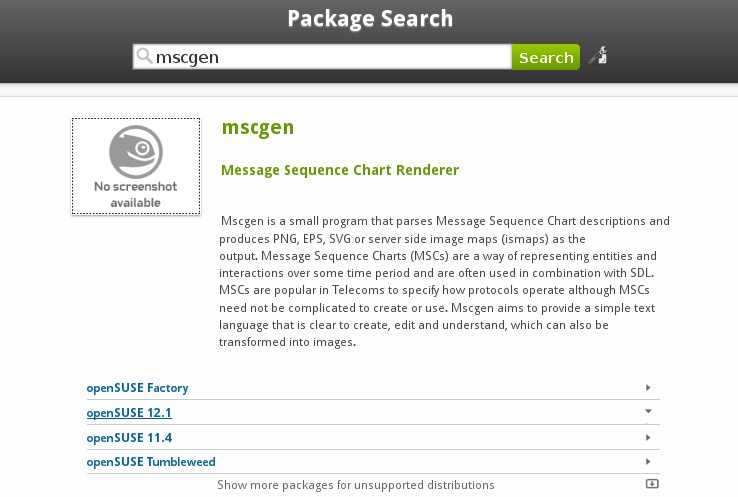
\includegraphics[width=0.5\textwidth]{images/write/graph/mscgen/install-OpenSuse-1}
	\caption[جستجوی نرم‌افزار \lr{mscgen} در موتور جستجوی \lr{OpenSuse}]{
		پس از جستجوی نرم‌افزار \lr{mscgen} و با استفاده از امکان‌های فراهم شده می‌توان
		به سادگی نرم‌افزاری مورد نظر را نصب و راه اندازی کنید.
	}
	\label{images/write/graph/mscgen/install-OpenSuse-1}
\end{figure}

همانگونه که در شکل \ref{images/write/graph/mscgen/install-OpenSuse-1} نمایش داده
شده است امکان نصب نرم‌افزار با تنها یک کلیک فراهم شده است. با انتخاب نرم‌افزار
برای نصب یک دریچه محاوره‌ای (که در شکل
\ref{images/write/graph/mscgen/install-OpenSuse-2} نمایش داده شده است) باز
می‌شود که اطلاعات ابتدایی مخزن نرم افزار را نمایش می دهد. پس از اطمینان یافتن از
مسیر و نوع مخزن دکمه \lr{Next} را کلیک کنید.

\begin{figure}
	\centering
	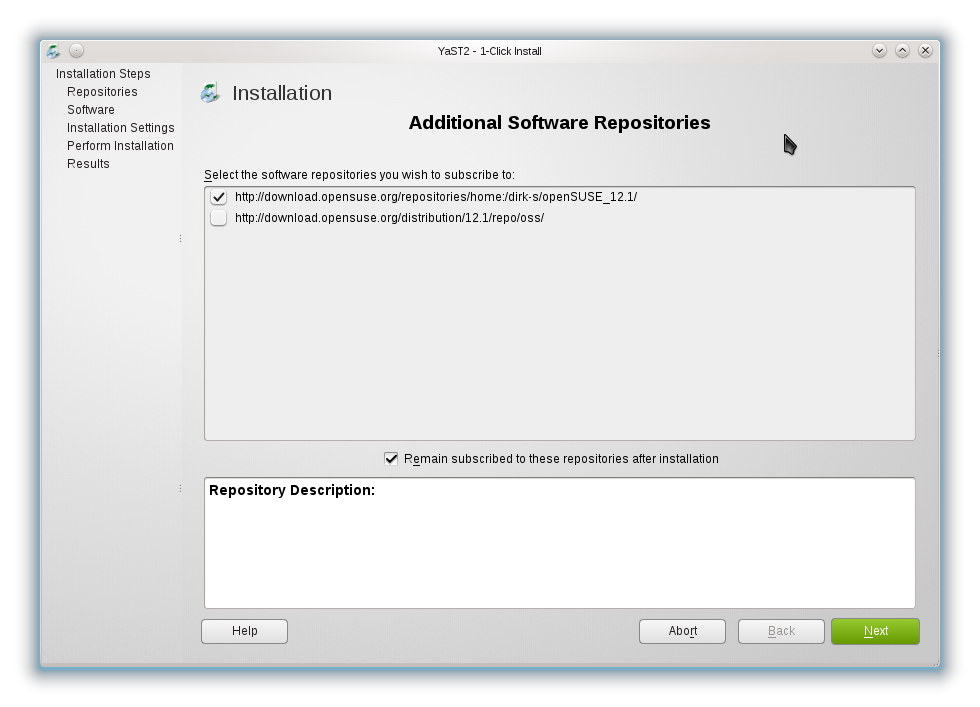
\includegraphics[width=0.5\textwidth]{images/write/graph/mscgen/install-OpenSuse-2}
	\caption[اطلاعات مخزن نرم‌افزاری برای نصب \lr{mscgen}]{
		در این دریچه محاوره‌ای علاوه بر نمایش آدرس، نوع مخزن نرم‌افزاری نیز نمایش داده
		می‌شود. پیش از نصب نرم‌افزار به آدرس و نوع آن توجه کنید.
	}
	\label{images/write/graph/mscgen/install-OpenSuse-2}
\end{figure}

در دریچه محاوره‌ای بعد اطلاعات بسته‌ نرم‌افزاری انتخاب شده برای نصب نمایش داده
می‌شود. این اطلاعات شامل نام و یک توصیف مختصر در مورد نرم افزار است. در شکل
\ref{images/write/graph/mscgen/install-OpenSuse-3} نیز اطلاعات و نام نرم‌افزار
\lr{mscgen} قابل مشاهده است. توجه داشته باشید که در این فهرست تنها همین
نرم‌افزار موجود بوده و برای نصب انتخاب شده باشد. پس از اطمینان حاصل کردن از
اطلاعات نرم‌افزار دکمه \lr{Next} را کلیک کنید.

\begin{figure}
	\centering
	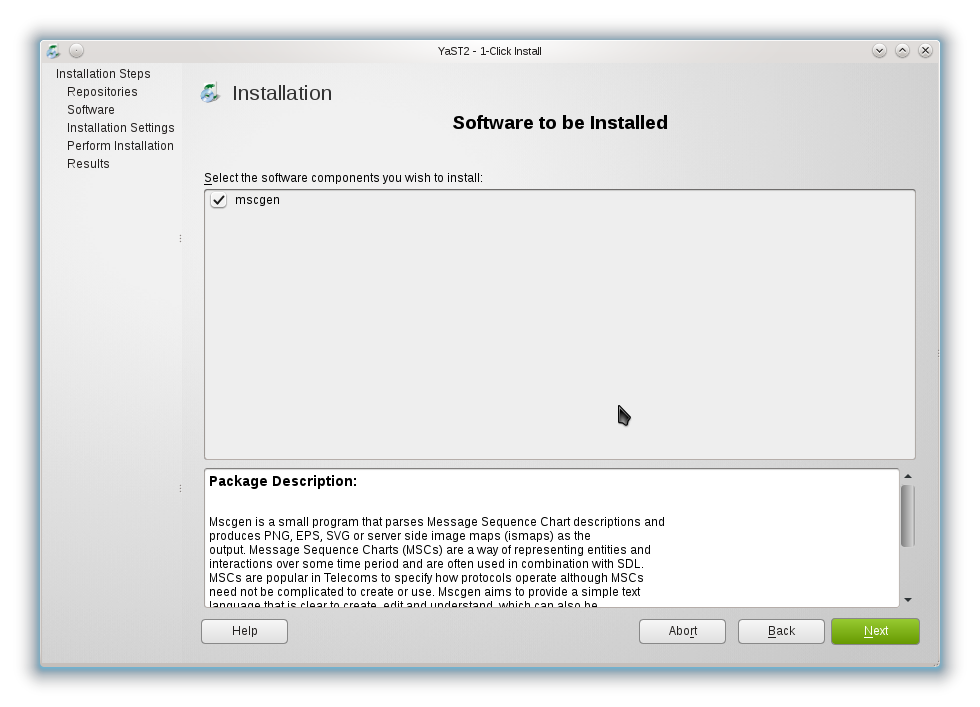
\includegraphics[width=0.5\textwidth]{images/write/graph/mscgen/install-OpenSuse-3}
	\caption[اطلاعات نرم‌افزار \lr{mscgen}]{
		در این دریچه محاوره‌ای اطلاعات کلی بسته \lr{mscgen} نمایش داده شده است. در بخش
		اول این دریچه محاوره‌ای فهرست نرم‌افزارها و در بخش انتهایی توضیحات نرم‌افزار
		انتخاب شده نمایش داده شده است.
	}
	\label{images/write/graph/mscgen/install-OpenSuse-3}
\end{figure}

پس از تایید مخزن‌های نرم‌افزاری و نرم افزارهای مورد نظر فرآیند نصب قابل اجرا
خواهد بود اما پیش از آن در یک دریچه محاوره‌ای خلاصه تمام اطلاعات برای تایید
نهایی نمایش داده می‌شود. همانگونه که در شکل \ref{images/write/graph/mscgen/install-OpenSuse-4}
نمایش داده شده است در این دریچه پایانی فهرستی از تمام داده‌های مورد استفاده در
فرآیند نصب نمایش داده می‌شود. در صورتی که این اطلاعات با اطلاعات مورد نظر شما
تطابق داشت دکمه \lr{Next} را برای ادامه فرآیند کلیک کنید.

\begin{figure}
	\centering
	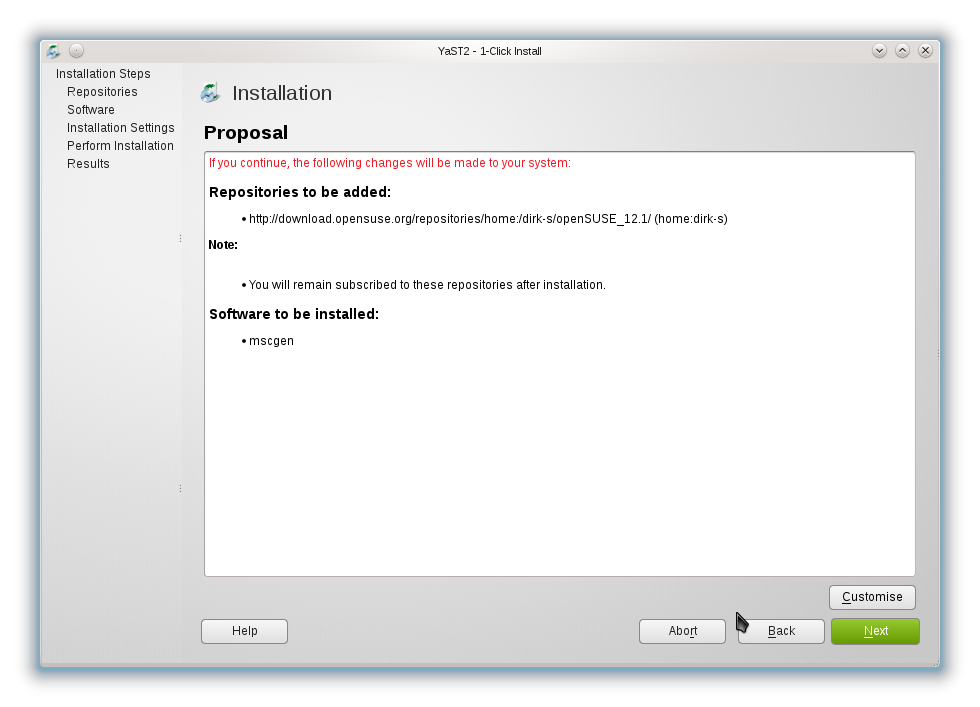
\includegraphics[width=0.5\textwidth]{images/write/graph/mscgen/install-OpenSuse-4}
	\caption[اطلاعات کلی فرآیند نصب نرم‌افزار \lr{mscgen}]{
		دریچه محاوره‌ای شامل تمام اطلاعات نرم افزارها و مخزن‌های مورد استفاده بوده و
		اخرین دریچه محاوره‌ای است که پیش از فرایند نصب نمایش داده می شود.
	}
	\label{images/write/graph/mscgen/install-OpenSuse-4}
\end{figure}

در سیستم‌های لینوکس کاربران سیستم اجازه نصب نرم‌افزار جدید را نداشته و تنها
کاربر اصلی سیستم می‌تواند یک نرم‌افزار جدید را در سیستم نصب کند. از این رو
اگر فرآیند نصب توسط یک کاربر عادی فراخوان شده باشد یک دریچه محاوره‌ای دیگر برای
دریافت گذرواژه نمایش داده می‌شود. در شکل
\ref{images/write/graph/mscgen/install-OpenSuse-5} این دریچه نمایش داده شده
است. گذرواژه کاربر ریشه را وارد و دکمه \lr{Ok} را کلیک کنید.

\begin{figure}
	\centering
	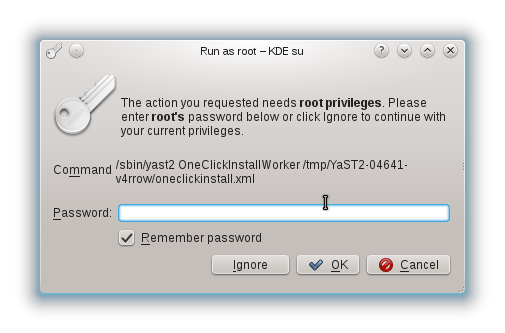
\includegraphics[width=0.5\textwidth]{images/write/graph/mscgen/install-OpenSuse-5}
	\caption[احراز اصالت برای نصب نرم‌افزار \lr{mscgen}]{
		در این دریچه محاوره‌ای علاوه بر بیان درخواست اصلی کاربر، از او خواسته می‌شود
		که گذرواژه کاربر اصلی را وارد کند. تنها کاربر اصلی سیستم می‌تواند نرم‌افزار
		جدید را در سیستم نصب کند.
	}
	\label{images/write/graph/mscgen/install-OpenSuse-5}
\end{figure}

در نهایت فرآیند نصب نرم‌افزار شروع خواهد شد. در این فرآیند نه تنها خود نرم‌افزار
بلکه بسته‌های مورد نیاز در آن \glspl{download} شده و نصب می‌شود. فرآیند و پیشرفت
نصب در یک دریچه محاوره‌ای نمایش داده می‌شود که در شکل
\ref{images/write/graph/mscgen/install-OpenSuse-6} نمایش داده شده است. با
استفاده از این دریچه محاوره‌ای نه تنها پیشرفت کار مشخص است بلکه امکان لغو آن نیز وجود دارد.

\begin{figure}
	\centering
	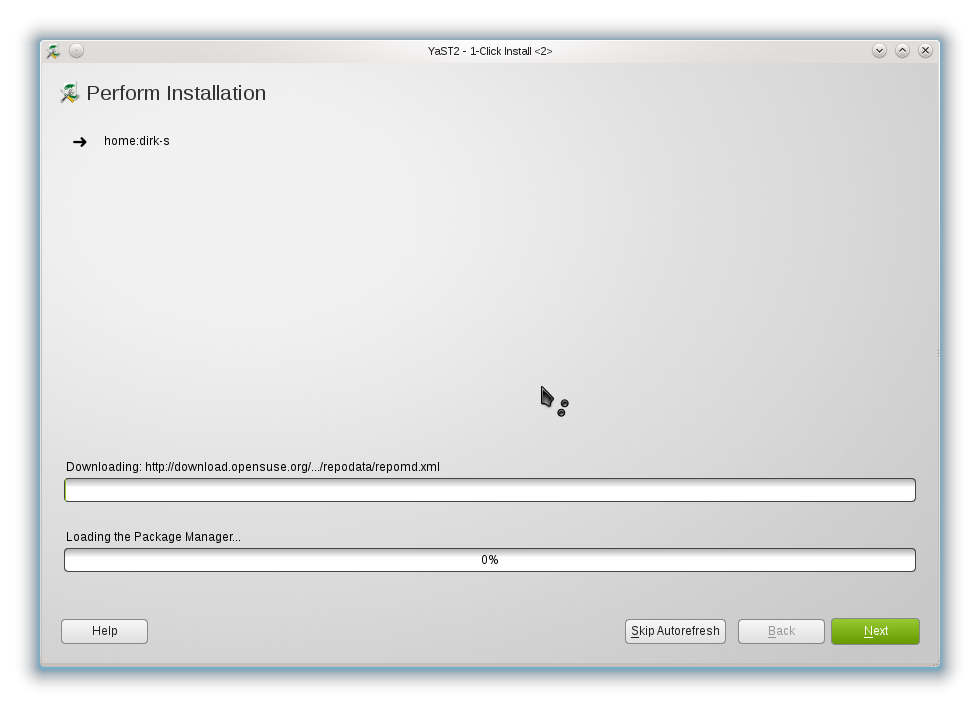
\includegraphics[width=0.5\textwidth]{images/write/graph/mscgen/install-OpenSuse-6}
	\caption[فرآیند نصب نرم‌افزار \lr{mscgen}]{
		در این دریچه محاوره‌ای نه تنها میزان پیشرفت کار نمایش داده شده بلکه امکان‌های
		جنبی مانند راهنما و لغو نصب نیز وجود دارد.
	}
	\label{images/write/graph/mscgen/install-OpenSuse-6}
\end{figure}

در پایان بسته‌های مورد نیاز و برنامه‌های احرایی نصب شده و دستورهای مناسب به
سیستم اضافه خواهد شد. برای بررسی نصب کامل این ابزار در \glspl{terminal program} دستور
\lr{mscgen} را وارد کنید. با صادر کردن این دستور در صورتی که نرم‌افزار به صورت
کامل نصب شده باشد خروجی زیر در \lr{terminal} نمایش داده می‌شود.

\begin{Shell}
> mscgen
-T <type> must be specified on the command line                                                         
Usage: mscgen -T <type> [-o <file>] [-i] <infile>                                                       
       mscgen -l                                                                                        

Where:                                                                                                  
 -T <type>   Specifies the output file type, which maybe one of 'png', 'eps',
             'svg' or 'ismap'
 -i <infile> The file from which to read input.  If omitted or specified as
              '-', input will be read from stdin.  The '-i' flag maybe
              omitted if <infile> is specified as the last option on the
              command line.
 -o <file>   Write output to the named file.  This option must be specified if 
              input is taken from stdin, otherwise the output filename
              defaults to <infile>.<type>.  This may also be specified as '-'
              to write output directly to stdout.
 -p          Print parsed msc output (for parser debug).
 -l          Display program licence and exit.

Mscgen version 0.20, Copyright (C) 2010 Michael C McTernan,
                                        Michael.McTernan.2001@cs.bris.ac.uk
Mscgen comes with ABSOLUTELY NO WARRANTY.  This is free software, and you are
welcome to redistribute it under certain conditions; type `mscgen -l' for
details.

PNG rendering by libgd, www.libgd.org
\end{Shell}

\subsubsection{ویندوز}

با توجه به محدودیت‌های موجود در سیستم‌های عمال ویندوز امکان نصب خودکار و به روز
رسانی وحود ندارد. از این رو ابتدا باید نرم‌افزار را \glspl{download} و سپس اقدام
به نصب آن کنید. در ادامه فرض شده است که برنامه نصب این ابزار در دست رس باشد.
برنامه نصب را به روی سیستم خود \glspl{copy} کرده و آن را احرا کنید. با اچرا شدن
برنامه یک دریچه محاوره‌ای همانند شکل \ref{images/write/graph/mscgen/install-win-1}
نمایش داده خواهد شد.
در این دریچه محاوره‌ای اطلاعات کلی نرم‌افزار نمایش داده شده است. دکمه \lr{Next}
را برای ادامه کار کلیک کنید.

\begin{figure}
	\centering
	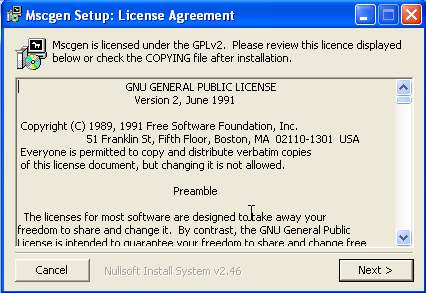
\includegraphics[width=0.5\textwidth]{images/write/graph/mscgen/install-win-1}
	\caption[اطلاعات کلی نرم‌افزار برای نصب در سیستم‌عامل ویندوز]{
		در این دریچه اطلاعاتی ابتدایی نمایش داده شده است. برای نمونه می‌توان به گواهی
		نامه آن اشاره کرد.
	}
	\label{images/write/graph/mscgen/install-win-1}
\end{figure}

در گام بعد دریچه محاوره‌ای برای تعیین پارامترهای مورد نیاز در فرآیند نصب نمایش
داده می‌شود. مهم‌ترین و تنها اطلاعاتی که در این گام باید تعیین شود مسیری است که
\glspl{installer program} داده‌ها را در آن ایجاد خواهد کرد. نمای کلی این دریچه
محاوره‌ای در شکل \ref{images/write/graph/mscgen/install-win-2}
نمایش داده شده است. دکمه \lr{Install} را کلیک کنید.

\begin{figure}
	\centering
	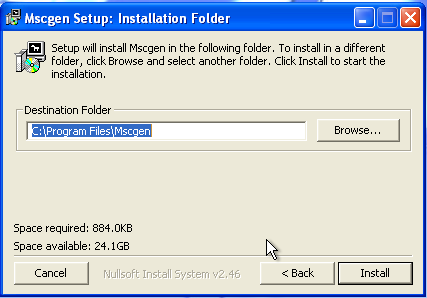
\includegraphics[width=0.5\textwidth]{images/write/graph/mscgen/install-win-2}
	\caption[تنظیم مورد نیاز برای نصب \lr{mscgen} در ویندوز]{
		تنها اطلاعات مورد نیاز برای نصب این نرم‌افزار تعیین مسبی نصب است. با استفاده
		از دکمه \lr{Brows} می‌توانید مسیر مورد نظر خود را تعیین کنید.
	}
	\label{images/write/graph/mscgen/install-win-2}
\end{figure}

در آخرین گام فرآیند نصب، فرآیند نصب آغاز شده و یک دریچه محاوره‌ای نمایش داده
می‌شود. همانگونه که در شکل \ref{images/write/graph/mscgen/install-win-3}
قابل مشاهده است در این دریچه پیشرفت فرایند نصب نمایش داده می‌شود.

\begin{figure}
	\centering
	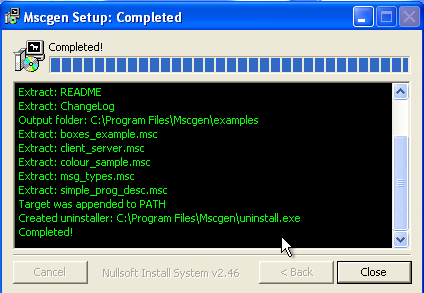
\includegraphics[width=0.5\textwidth]{images/write/graph/mscgen/install-win-3}
	\caption[پیشرفت فرآیند نصب \lr{mscgen} در ویندوز]{
		در این دریچه محاوره‌ای میزان پیشرفت فرآیند نصب نمایش داده می‌شود. پس از پایان
		فرایند نصب دکمه \lr{Close} فعال می‌شود تا با استفاده از آن به فرآیند نصب خاتمه
		داده شود.
		}
	\label{images/write/graph/mscgen/install-win-3}
\end{figure}

در نهایت پس از پایان یافتن این مراحل این ابزار در سیستم نصب شده و قابل استفاده
می‌باشد در اینجا نیز باید دستور \lr{mscgen} به سیستم اضافه شده باشد. برای
اطمینان از این موضوع یک \lr{CMD} باز کرده و در آن این دستور را فراخوانی کنید. با
فراخوانی کردن این دستور باید داده‌های زیر در خروچی نمایش داده شود.

\begin{Shell}
C:\Documents and Settings\malek>mscgen
-T <type> must be specified on the command line
Usage: mscgen -T <type> [-o <file>] [-i] <infile>
       mscgen -l

Where:
 -T <type>   Specifies the output file type, which maybe one of 'png', 'eps',
             'svg' or 'ismap'
 -i <infile> The file from which to read input.  If omitted or specified as
              '-', input will be read from stdin.  The '-i' flag maybe
              omitted if <infile> is specified as the last option on the
              command line.
 -o <file>   Write output to the named file.  This option must be specified if
              input is taken from stdin, otherwise the output filename
              defaults to <infile>.<type>.  This may also be specified as '-'
              to write output directly to stdout.
 -p          Print parsed msc output (for parser debug).
 -l          Display program licence and exit.

Mscgen version 0.20, Copyright (C) 2010 Michael C McTernan,
                                        Michael.McTernan.2001@cs.bris.ac.uk
Mscgen comes with ABSOLUTELY NO WARRANTY.  This is free software, and you are
welcome to redistribute it under certain conditions; type `mscgen -l' for
details.

PNG rendering by libgd, www.libgd.org
\end{Shell}

در این حالت این ابزار در سیستم نصب شده و در درسترس دیگر ابزارها برای تولید مستند
قرار دارد.

\subsection{\lr{Graphviz}}

\lr{Graphviz} روشی برای نمایش داده‌های ساختار یافته به صورت نمودار و گراف است.
از آنجا که بسیاری از شاخه‌های علوم همواره با داده‌های ساختار یافته در ارتباط
بوده و نمایش داده‌ها از اهمیت خاصی برخوردار است، \lr{Graphviz} به عنوان یک ابزار
بسیار کاربردی در انها مطرح است. از این میان می‌توان با شبکه،
\glspl{bioinformatics}، مهندسی رایانه، ساختمان داده، طراحی \glspl{web}،
\glspl{machine learning} و بسیاری دیگر اشاره کرد.

این نرم‌افزار یک نرم‌افزار \glspl{open source} بوده و به روی سکوهای متفاوتی
مانند لینوکس و ویندوز قابل استفاده است. این نرم‌افزار از لایه بندی‌های متفاوتی
برای ترسیم گراف‌ها، به صورت پیش فرض استفاده می‌کند. از طرفی ابزارهای مناسبی برای
کار به روی \glspl{web}، کتابخانه‌ها، زبان‌های برنامه سازی فراهم شده است.

روال کلی این نرم‌افزار به این صورت است که در ابتدا کاربر با استفاده از زبان‌های
ساده و متنی گراف و نمودار خود را توصیف می‌کند، پس از آن این توصیف با استفاده از
این ابزار به صورت یک نمایش و نمودار تبدیل شده و در قالب‌های متفاوتی مانند
\gls{SVG}، \gls{PDF} و یا قالب‌های دیگر ذخیره می‌شود.

توانایی به کارگیر تنظیم‌های متفاوت مانند رنگ، قلم، لایه بندی، طرح خط‌ها،
نمایش‌ها و دیگر موارد این ابزار را به یک ابزار بسیار کاربردی در طراحی و ایجاد
نمودارها مبدل ساخته است.

در عمل این ابزار به گونه‌ای طراحی شده است که داده‌های ساختار یافته را به عنوان
داده ورودی دریافت کرده و بر اساس دستورهای خاص آنها را ترسیم کند اما این به آن
معنی نیست که قادر به ترسیم نمودارهای دیگر نباشد. به بیان دیگر این امکان نیز
فراهم شده است که کاربر تنها نمایش و ترسیم را تعیین کرده و داده‌های ورودی مورد
نظر خود را به عنوان پارامتر در آن وارد کند.

در این بخش روش نصب و به کار گیری ابن نرم‌افزار به روی سکوهای متفاوتی مانند
لینوکس و ویندوز تشریح خواهد شد و در ادامه روش به کارگیر این نرم‌افزار در مستند
سازی تکنیکی مورد بررسی قرار خواهد گرفت.

\subsubsection{لینوکس}
در این قسمت به نحوه نصب \lr{Graphviz} بر روی سیستم عامل لینوکس با توزع \lr{SUSE} اشاره خواهد شد.
مانند روش نصب همه نرم افزارها و بسته‌های مورد استفاده در لینوکس، جهت نصب \lr{Graphviz} نیز ابتدا مانند شکل زیر باید به بخش مدیریت نرم افزارها در لینوکس رفت.

\begin{figure}
	\centering
	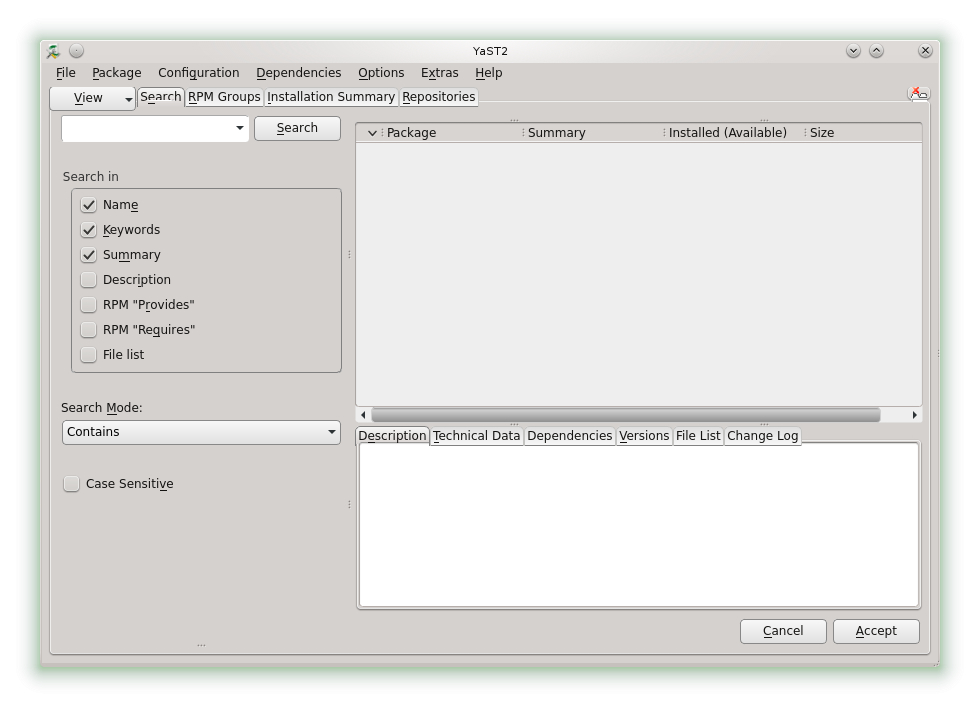
\includegraphics[width=0.5\textwidth]{images/write/graph/graphviz/install-OpenSUSE-0}
	\caption[]{بخش مدیریت نرم افزارها در لینوکس}
	\label{images/write/graph/graphviz/install-OpenSUSE-0}
\end{figure}

در قسمت جستجوی نرم افزار مورد نظر نام \lr{Graphviz} را وارد کنید. همانطورد که در پنجره سمت راست حاصل از نتایج جستجو دیده می‌شود تمام نرم افزارها و بسته‌های مختلف حاصل مربوط به کلمه فوق دیده می‌شود. با انتخاب \lr{Graphviz} و علامت زدن آن، نرم افزار مورد نظر و تمام بسته‌های مورد نیاز در سیستم نصب می‌شوند.
\begin{figure}
	\centering
	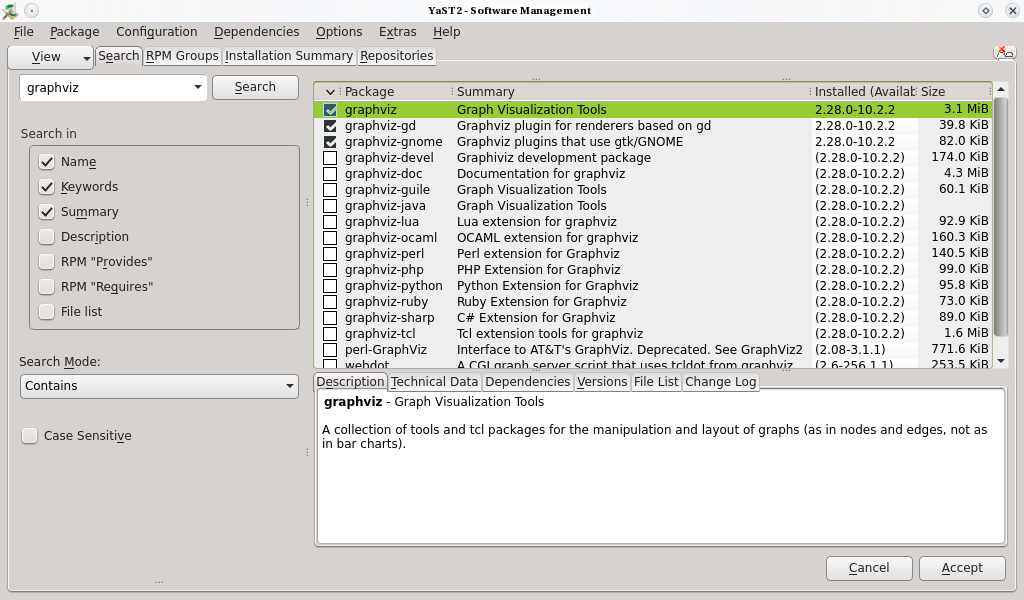
\includegraphics[width=0.5\textwidth]{images/write/graph/graphviz/install-OpenSUSE-1}
	\caption[]{بخش جستجو و نصب نرم افزار مورد نظر
	
	}
	\label{images/write/graph/graphviz/install-OpenSUSE-1}
\end{figure}
در انتها فرایند نصب نرم افزار و تمام بسته‌های مورد نیاز نرم افزار تا پایان نصب انجام می‌شود.
\begin{figure}
	\centering
	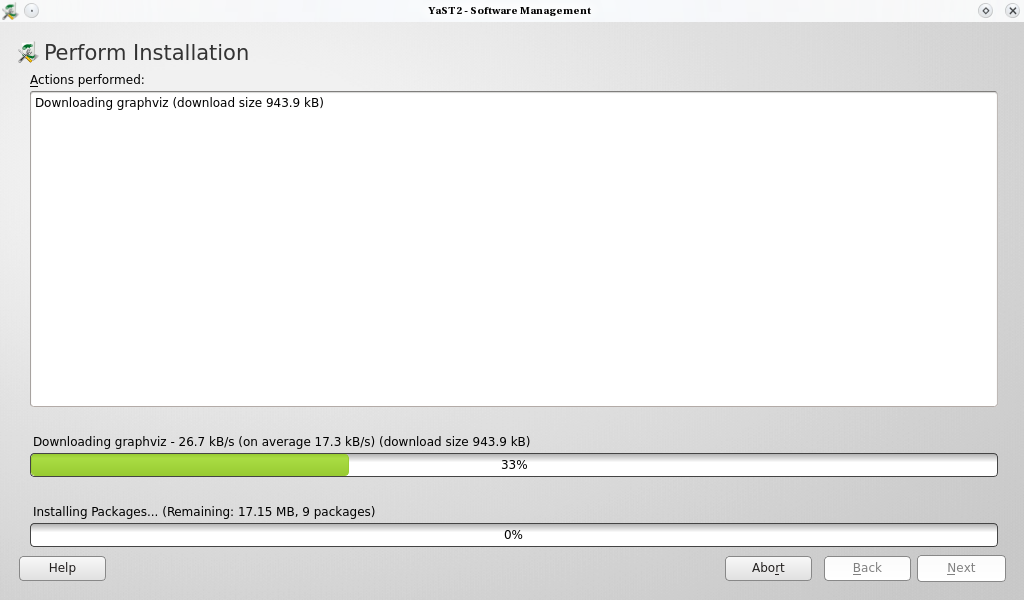
\includegraphics[width=0.5\textwidth]{images/write/graph/graphviz/install-OpenSUSE-2}
	\caption[]{فرآیند نصب نرم افزار
	
	}
	\label{images/write/graph/graphviz/install-OpenSUSE-2}
\end{figure}

\subsubsection{ویندوز}

\begin{webreference}
جهت نصب \lr{Graphviz} بر روی سیتم عامل ویندوز ابتدا باید نرم افزار را دانلود کرد
و سپس آن را نصب کرد. می‌توانید نرم افزار را از سایت زیر دانلود کنید:
\begin{latin}
http://www.graphviz.org/Download\_windows.php
\end{latin}
\end{webreference}

پس از دانلود نرم افزار فوق بر روی آن دوبار کلیک کنید تا فرآیند نصب نرم افزار
شروع شود. در پنجره ظاهر شده اطلاعات کلی از نرم افزار آمده است. برای ادامه روند
نصب بر روی کلید \lr{next} کلیک کنید.

\begin{figure}
	\centering
	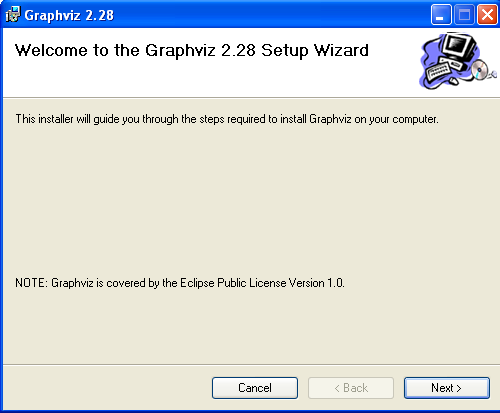
\includegraphics[width=0.5\textwidth]{images/write/graph/graphviz/install-1}
	\caption[]{صفحه اولیه نصب نرم افزار در ویندوز
	
	}
	\label{images/write/graph/graphviz/install-1}
\end{figure}

در پنجره بعد باید مسیری برای نصب نرم افزار انتخاب کرد. همچنین سطح دسترسی برای
استفاده از نرم افزار را مشخص کرده و روند نصب را ادامه داد.

\begin{figure}
	\centering
	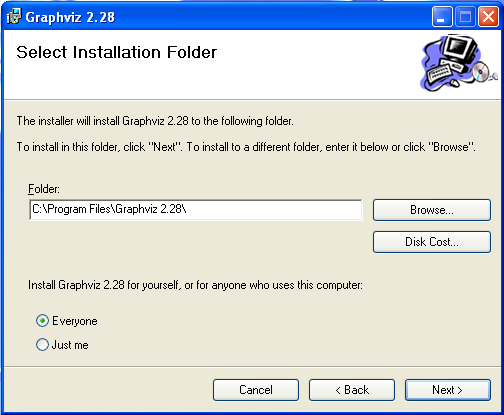
\includegraphics[width=0.5\textwidth]{images/write/graph/graphviz/install-2}
	\caption[]{انتخاب مسیر جهت نصب نرم افزار
	
	}
	\label{images/write/graph/graphviz/install-2}
\end{figure}

در ادامه نصب باید مرحله نصب نهایی نرم افزار را تصدیق کرد تا نرم افزار شروع به
نصب شود. در آخر کلید \lr{close} را جهت اتمام نصب نرم افزار کلیک کنید.
\begin{figure}
	\centering
	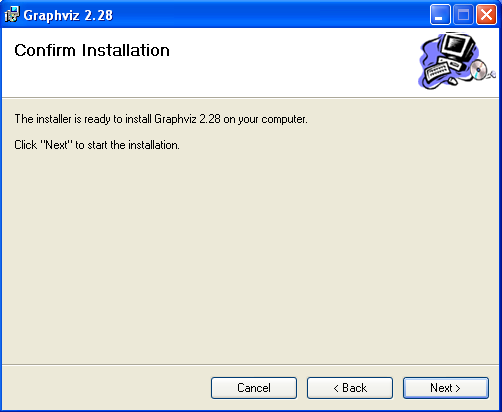
\includegraphics[width=0.5\textwidth]{images/write/graph/graphviz/install-3}
	\caption[]{تایید نهایی نصب نرم افزار
	
}
	\label{images/write/graph/graphviz/install-3}
\end{figure}

پس از نصب کامل برنامه از منوی \lr{start} برنامه نصب شده \lr{GVEdit.exe} را اجرا
کرده تا ویزارد مربوط به \lr{Graphviz} ظاهر شود. در این ویزارد با ایجاد یک پروژه
جدید و در پنجره‌ای که با نام پروژه ظاهر شده است می‌توان کدهای گراف مورد نظر را
اجرا کرد. پس از تکمیل کد نهایی با زدن کلید \lr{F5} صفحه کلید نتیجه کد نوشته شده
در پنجره جداگانه نمایش داده می‌شود که می‌توان آن را در قالب‌های مختلف ذخیره کرد.




%%
% حق نشر 1390-1402 دانش پژوهان ققنوس
% حقوق این اثر محفوظ است.
% 
% استفاده مجدد از متن و یا نتایج این اثر در هر شکل غیر قانونی است مگر اینکه متن حق
% نشر بالا در ابتدای تمامی مستندهای و یا برنامه‌های به دست آمده از این اثر
% بازنویسی شود. این کار باید برای تمامی مستندها، متنهای تبلیغاتی برنامه‌های
% کاربردی و سایر مواردی که از این اثر به دست می‌آید مندرج شده و در قسمت تقدیر از
% صاحب این اثر نام برده شود.
% 
% نام گروه دانش پژوهان ققنوس ممکن است در محصولات دست آمده شده از این اثر درج
% نشود که در این حالت با مطالبی که در بالا اورده شده در تضاد نیست. برای اطلاع
% بیشتر در مورد حق نشر آدرس زیر مراجعه کنید:
% 
% http://dpq.co.ir/licence
%
\section{\lr{Mscgen}}

همانگونه که پیش از این اشاره شده با استفاده از این ابزار می‌توان \glspl{message
sequence chart} را در مستند‌ها ایجاد کرد و به خوانایی مستند‌های ایجاد شده افزود.
یک \glspl{message sequence chart} را در مستند می‌توان به دو روش متفاوت ایجاد
کرد. در روش اول با استفاده از برچسب \lr{msc} می‌توان در لابه‌لای مستندهای تکنیکی
نوشته شده نمودارها مورد نیاز ایجاد کرد. استفاده از این دستور امکان بیان جزئیات
کامل \glspl{message sequence chart} را در خود مستند فراهم می‌کند. ساختار کلی این
دستور به صورت زیر است.
 
\begin{C++}
/**
 * \msc
 * [Diagram detail]
 * \endmsc
 */
\end{C++}

با استفاده از این قالب، قمست مستند ایجاد شده به عنوان یک توصیف صحیح از یک
\glspl{message sequence chart} در نظر گرفته می‌شود. همانگونه که این قالب کلی
قابل مشاهده است توصیف نمودار می‌بایست در محدوده ایجاد شده دو دستور \lr{msc} و
\lr{endmsc} قرار گیرد. قراردادهای توصیف نمودار در انتهای این بخش مورد بررسی قرار
گرفته شده است.

\begin{note}
برای استفاده از این دستورها باید بر اساس قراردادها و زبان توصیف نمودار، \glspl{}
را به صورت کامل و بدون اشتباه در میان این دو دستور نوشته شود. در صورتی که
اشتباهی در این توصیف وجود داشده باشد \glspl{documenter} از آن صرف نظر خواهد کرد.
\end{note}

برای نمونه فرض کنید که قراردادی وجود دارد که در آن یک طرف دستوری را ارسال کرده و
دیگری نتیجه اجرای دستور را گزارش می‌دهد. نمودار این قرارداد در نمونه زیر ایجاد
شده است.

\begin{C++}
/**
 * \msc
 * Sender,Receiver;
 * Sender->Receiver [label="Command()"];
 * Sender<-Receiver [label="Ack()"];
 * \endmsc
 */
\end{C++}

با یک دید نه تنها می‌توان مفاهیم به کار رفته در این توصیف را درک کرد بلکه به این
نکته اذعان کرد که توصیف نمودار بسیار شبه به همان توصیف قرارداد خواهد بود. این
شباهت در توصیف یک قرارداد و توصیف نمودار آن یکی از مهم‌ترین خصوصیت‌های این دستور
است.

% maso 1391: تنظیم‌های کلی برای استفاده از دستور

فرآیند کلی تولید یک \glspl{message sequence chart} با استفاده از این دستور به
این قرار است: در گام نخست کاربر توصیف کامل نمودار را در مستند ایجاد کرده و
\lr{Doxygen} را برای تولید مستند نهایی فراخوانی می‌کند، \glspl{documenter} با
مشاهده این دستور توصیف نمودار را استخراج کرده و با استفاده از ابزار \lr{mscgen}
آن را به \glspl{message sequence chart} معادل ترجمه می‌کند و در نهایت نمودار
ایجاد شده را در مستند نهایی ایجاد شده قرار می‌گیرد. در این فرآیند
\glspl{documenter} با استفاده از ابزار جانبی \lr{mscgen} نمودارهای مورد نیاز
کاربر را ایجاد کرده و در در فرآیند تولید مستند نهایی استفاده می‌کند از این رو
باید روشی برای فراخوانی و استفاده از این ابزار برای \glspl{documenter} فراهم
شود. زمانی که ابزار \lr{mscgen} به صورت سیستمی نصب شده باشد و دستور آن به عنوان
یک دستور جدید در کل سیستم قابل دسترسی باشد \lr{Doxygen} به صورت خودکار آن را
تشخیص داده و از آن استفاده می‌کند، اما مشکل اساسی زمانی رخ می‌دهد که این ابزار
به صورت محلی نصب شده و به عنوان یک دستور معرفی نشده باشد. در این حالت با استفاده
از گزینه \lr{MSCGEN\_PATH} می‌توان مسیر این ابزار را برای \glspl{documenter}
تعیین کرد. حالت کلی استفاده از این گزینه در تنظیم‌های مستند به صورت زیر است:

\begin{Shell}
MSCGEN_PATH = <path to mscgen>
\end{Shell}

زمانی که این خصوصیت در پیکره بندی مستند تعریف نشده باشه \glspl{documenter} به
صورت خودکار در مسیرهای استاندارد به دنبال این ابزار جستجو خواهد کرد.

%maso 1391: استفاده از پرونده به عنوان نمودار
اما استفاده از دستور \lr{msc} و توصیف نمودار در خود مستند تنها روش ایجاد
\glspl{message sequence chart} نیست. یک روش بسیار مناسب و پرکاربرد توصیف نمودار
در پرونده‌های جداگانه و استفاده از دستور \lr{mscfile} است. با استفاده از این
دستور می‌توان یک پرونده شامل توصیف یک نمودار را به مستند اضافه کرد. ساختار کلی
این دستور به صورت زیر است:

\begin{C++}
 /**
  * \mscfile <file> ["caption"]
  */
\end{C++}

نخستن پارامتر ورودی این برچسب مسیر پرونده‌ای را که توصیف نمودار در
آن ایجاد شده است و پارامتر دوم زیر نویس نمودار ایجاد شده را تعیین
می‌کنند. پرونده تعیین شده به عنوان نمودار باید در مسیرهایی ایجاد شده باشد که در
پرونده پیکره بندی مشخص شده است. تعیین مسیر پرونده‌های مورد استفاده در این دستور
با استفاده از برچسب \lr{MSCFILE\_DIRS} در پرونده پیکره بندی تعیین می‌شود.

\begin{note}
مسیر پرونده در این دستور نمی‌تواند شامل \glspl{space} باشد، در این حالت مسیر را
باید در میان کوتیشن نوشت. این روش در حالت کلی به صورت زیر است:
\begin{C++}
 /**
  * \mscfile "<file path>" ["caption"]
  */
\end{C++}
\end{note}

%TODO: maso 1391: تنظیم‌های پرونده‌ها

% TOTO: hadi 1391: در مورد ساختار کلی توصیف نمودار
% TOTO: hadi 1391: در مورد نوشتن توضیحات در متن کدهای mscgen

\subsection{موجودیت‌ها}

% arcskip
% IDURL
% ID
% URL
% label

% Lists the entities that will be used in the message sequence chart, in the order
% in which they should appear left to right and horizontally across the page. Note
% that each entity name can or may not be quoted, unless the name is to include a
% space, in which case double quotes are required.
% 
% 
% arctextbgcolour, arctextbgcolor
% arctextcolour, arctextcolor
% arclinecolour, arclinecolor

هر موجودیت در سیستم می‌تواند به موجودیت‌های دیگر سیستم پیام بدهد یا پیامی از
آن‌ها دریافت کند. در واقع موجودیت‌ها نقش اصلی را در \glspl{message sequence
chart} دارند. بنابراین قبل از هر کاری باید موجودیت‌های نمودار را تعیین کرد. برای
تعریف یک موجودیت در نمودار کافی است نام مورد نظر برای موجودیت را بنویسید و پس از
آن یک علامت نقطه ویرگول ($;$) قرار دهید. برای تعریف چند موجودیت هم باید از کاما
استفاده شود. نکته مهم اینکه تعریف موجودیت‌ها را نباید با نقطه ویرگول از هم جدا
کرد و فقط بعد از آخرین موجودیت علامت نقطه ویرگول گذاشته می‌شود. در نموداری که
توسط ابزار \lr{Mscgen} تولید می‌شود موجودیت‌ها از سمت چپ به راست و به همان
ترتیبی که در هنگام تعریف آورده شده‌اند قرار می‌گیرند. در کد زیر نحوه تعریف
موجودیت‌ها نشان داده شده است:

\begin{MSC}
msc {
	entity1, entity2, ... ,	entityn;
	
	# Definition of message(s)
	
}
\end{MSC}

در این کد به تعداد دلخواه موجودیت تعریف کرده‌ایم. همانطور که به راحتی می‌توان از
کد فهمید برای تعریف هر موجودیت کافی است نامی که می‌خواهیم به موجودیت بدهیم را
بیان کنیم. فرض کنید نموداری را به صورت زیر توصیف کرده باشیم:

\begin{MSC}
msc {
	e1, e2, e3;
	
	e1->e2;	
}
\end{MSC}

در تصویر \ref{images/write/graph/mscgen/entity-example-1} نمایی از آنچه توسط
ابزار \lr{Mscgen} برای کد بالا تولید می‌شود نشان داده شده است. توجه شود که در کد
مربوط به این تصویر تنها سه موجودیت را تعریف کرده‌ایم و در نمودار تولید شده
موجودیت‌ها از چپ به راست با همان ترتیبی که در تعریف آمده‌اند قرار گرفته‌اند.

\begin{note}
دستور $e1->e2$ توصیف یک پیام از موجودیت \lr{e1} به موجودیت \lr{e2} است که در 
تصویر \ref{images/write/graph/mscgen/entity-example-1} نیز یک فلش از موجودیت اول
به موجودیت دوم دیده می‌شود.در قسمت~\ref{sec:message} انواع پیام‌ها و توصیف آن‌ها
به طور کامل شرح داده شده است.
در اینجا فقط برای اینکه بتوانیم نمودار مورد نظر را تولید کنیم یک پیام را تعریف کرده‌ایم
چون همانطور که قبلا گفته شد در توصیف نمودار باید حداقل یک موجودیت و حداقل یک پیام تعریف شده باشد.
در غیر این صورت ابزار \lr{Mscgen} با خطا مواجه شده و نمودار مربوطه را تولید نمی‌کند.
\end{note}

\begin{figure}[h]
	\centering
	\includegraphics[width=0.85\textwidth]{images/write/graph/mscgen/entity-example-1}
	\caption[مثالی از نحوه نمایش موجودیت‌ها توسط ابزار \lr{Mscgen}]
	{در این شکل سه موجودیت تعریف شده است. ابزار \lr{Mscgen} برای کد تعریف کننده این موجودیت‌ها 
	تصویری به این صورت نشان می‌دهد.}
	\label{images/write/graph/mscgen/entity-example-1}
\end{figure}

\begin{note}
موجودیت در \lr{UML} با عنوان \lr{life time} شناخته می‌شود.
\end{note}

اگر در نامی که می‌خواهید برای موجودیت خود بگذارید خط فاصله (فضای خالی) وجود
داشته باشد باید نام مورد نظر را بین دو علامت گیومه (\lr{"}) قرار دهید. مثلا فرض
کنید بخواهیم موجودیت‌هایی با نام‌های \lr{Entity One} و \lr{Entity Two} تعریف
کنیم برای این کار باید کد زیر را بنویسید:

\begin{MSC}
msc {
	"Entity One", "Entity Two";
	
	# Defenition of message(s)
}
\end{MSC}

حال فرض کنید نامی طولانی برای موجودیت خود گذاشته‌اید. در این صورت هر بار بخواهید
به این موجودیت ارجاعی داشته باشید (مثلا رابطه‌ای بین آن و یک موجودیت دیگر برقرار
کنید) مجبورید نام آن موجودیت را به طور کامل بیان کنید. به کد زیر توجه کنید:

\begin{MSC}
msc {
	"Entity Number one", "Entity Number two";
	
	"Entity Number one"->"Entity Number two";
}
\end{MSC}

خروجی ابزار \lr{Mscgen} برای این کد در تصویر
\ref{images/write/graph/mscgen/entity-example-2} نشان داده شده است.

\begin{figure}[h]
	\centering
	\includegraphics[width=0.85\textwidth]{images/write/graph/mscgen/entity-example-2}
	\caption[مثالی از نحوه تعریف موجودیت‌هایی با نام‌های طولانی و حاوی خط فاصله]
	{در این شکل خروجی ابزار \lr{Mscgen} برای کد مربوط به تعریف موجودیت‌هایی با نام طولانی نشان داده شده است.}
	\label{images/write/graph/mscgen/entity-example-2}
\end{figure}

برای پرهیز از این کار روش دیگری برای تعریف موجودیت وجود دارد. در این روش یک
موجودیت به همراه یک برچسب خاص تعریف می‌شود. نمونه‌ای از این روش تعریف موجودیت در
کد زیر آورده شده است:

\begin{MSC}
msc {
	a[label="Entity Number one"], b[label="Entity Number two"];
	
	a->b;
}
\end{MSC}

همانطور که در کد بالا دیده می‌شود دستور تعریف موجودیت به این صورت است: ابتدا
نامی که می‌خواهید qبرای ارجاعات بعدی در کد از آن استفاده کنید، سپس بین دو کروشه
ابتدا کلمه \lr{label}، سپس علامت مساوی (=) و در مقابل آن نامی که می‌خواهید در
دیاگرام تولیدی توسط ابزار \lr{Mscgen} برای موجودیت مورد نظر ظاهر شود. در واقع با
این کار برای موجودیت‌ها خصوصیت \lr{label} را تعریف کرده و مقداردهی می‌کنید. در این
روش هم برای تعریف چند موجودیت باید از کاما استفاده کرد و در انتهای تعریف
موجودیت‌ها نقطه‌ویرگول قرار داده شود.

نمودار مربوط به کد اخیر دقیقا مثل نمودار کد قبلی (تصویر
\ref{images/write/graph/mscgen/entity-example-2}) است. اما مشاهده می‌شود که
تعریف پیام‌ها در کد دوم چقدر ساده‌تر و سریع‌تر از کد قبل است.

% TODO: hadi 1391: تعریف خصوصیات مربوط به یک موجودیت
یک موجودیت علاوه بر خصوصیت \lr{label} خصوصیات دیگری نیز دارد که می‌توان آن‌ها را با
مقادیر دلخواه مقداردهی کرد. با خصوصیات مختلف یک موجودیت می‌توان موادی چون رنگ متن
مربوط به نام موجودیت، رنگ پس‌زمینه نام موجودیت، رنگ خط زمانی یا همان
\lr{time-line} موجودیت و \lr{\ldots} را تعیین کرد. به طور کلی برای مقداردهی
خصوصیات مختلف یک موجودیت باید هنگام تعریف موجودیت در مقابل نام آن و بین دو علامت کروشه
([]) خصوصیت مورد نظر را ذکر کرده و مقداری دلخواه خود را به آن خصوصیت بدهید. خصوصیات مختلف
باید با کاما از یکدیگر جدا شوند. شکل کلی مقداردهی به خصوصیات یک موجودیت به این صورت
است:

\begin{MSC}
msc {
	entity1[attribute1="value1" , attribute2="value2" , ... ,
	attribute="value"],
	entity2[attribute1="value1", attribute2="value2", ... ,
	attribute="value"];
	.
	.
	# Definition of messages
	.
	.
}
\end{MSC}

با استفاده از خصوصیت \lr{linecolor} یا \lr{linecolour} می‌توان رنگ خط زمانی
موجودیت را به رنگ دلخواه تغییر داد. با استفاده از خصوصیت \lr{textcolor} یا
\lr{textcolour} نیز می‌توان رنگ متن مربوط به نام موجودیت را تغییر داد و
با استفاده از خصوصیت \lr{textbgcolor} یا \lr{textbgcolour} می‌توان رنگ پس‌زمینه
نام موجودیت را تعیین کرد. لازم به ذکر است که این خصوصیات برای پیام‌ها نیز تعریف
تعریف شده که در بخش~\ref{sec:message} شرح داده شده‌اند. به کد زیر و تصویر معادل
تولید شده توسط ابزار \lr{Mscgen} برای این کد (تصویر \ref{images/write/graph/mscgen/entity-example-3}) توجه نمایید.

\begin{MSC}
msc {
	 a[label="Entity A", linecolor="green", textcolor="red", textbgcolor="yellow"],
	 b[label="Entity B", linecolor="blue", textcolor="#800000", textbgcolor="#c0c0c0"],
	 c[label="Entity C"];
	 
	 a->b;
  	 b->c;
  	 c->c;
  	 a<-c;
  	 a<-b;
}
\end{MSC}

\begin{figure}[h]
	\centering
	\includegraphics[width=0.85\textwidth]{images/write/graph/mscgen/entity-example-3}
	\caption[مثالی از نحوه تعریف خصوصیات مختلف موجودیت‌ها]
	{در این شکل خروجی ابزار \lr{Mscgen} برای کد مربوط به تعریف خصوصیات
	مختلف رنگی موجودیت‌ها نشان داده شده است.}
	\label{images/write/graph/mscgen/entity-example-3}
\end{figure}
 
رنگ قسمت‌های مختلف کلیه پیام‌هایی که از یک موجودیت شروع می‌شوند را نیز می‌توان
در خصوصیات مربوط به همان موجودیت کنترل کرد. با استفاده از خصوصیت
\lr{arclinecolor} یا \lr{arclinecolour} یک موجودیت می‌توان رنگ پیکان تمام
پیام‌هایی که از آن موجودیت شروع می‌شوند را تعیین کرد. به عبارتی با تعیین رنگ
برای این خصوصیت از موجودیت، رنگ پیش‌فرض تمام پیکان‌هایی که از آن موجودیت شروع
می‌شوند را تعیین کرده‌اید. البته می‌توان با تعیین خصوصیت \lr{linecolor} از یک
پیام خاص، رنگ آن پیکان آن پیام را تغییر داد تا از این رنگ پیش‌فرض استفاده نکند.
علاوه بر آن با استفاده از خصوصیت \lr{arctextcolor} یا \lr{arctextcolour} نیز
می‌توان رنگ متن پیام‌هایی که از یک موجودیت شروع می‌شوند را تغییر داد (رنگ متنی
که معمولا در بالای پیکان مربوط به یک پیام قرار می‌گیرد). در این مورد هم با تعیین
رنگ برای این خصوصیت از موجودیت، رنگ متن تمام پیام‌هایی که از آن موجودیت ارسال
می‌شوند را به صورت پیش‌فرض تعیین کرده‌اید.در مورد این خصوصیت هم می‌توان با تعیین
خصوصیت \lr{textcolor} از یک پیام خاص، رنگ متن آن پیام را تغییر داد تا از این رنگ
پیش‌فرض استفاده نکند. همچنین با استفاده از خصوصیت \lr{arctextbgcolor} یا \lr{arctextbgcolour} می‌توان رنگ
پس‌زمینه متن پیام‌هایی که از یک موجودیت شروع می‌شوند را مشخص کرد (رنگ پس‌زمینه
متنی که معمولا در بالای پیکان مربوط به یک پیام قرار می‌گیرد). با تعیین
رنگ برای این خصوصیت از موجودیت، رنگ پس‌زمینه متن تمام پیام‌هایی که از آن موجودیت ارسال می‌شوند را به
صورت پیش‌فرض تعیین کرده‌اید. باز هم می‌توان با تعیین خصوصیت \lr{textbgcolor} از
یک پیام خاص، رنگ پس‌زمینه متن آن پیام را تغییر داد تا از این رنگ پیش‌فرض استفاده
نکند. در زیر یک نمونه کد مثال برای دستکاری این خصوصیات آورده شده است. نمودار
متناظر این کد در تصویر \ref{images/write/graph/mscgen/entity-example-4} آورده
شده است.

\begin{MSC}
msc {
	 a[label="Entity A", arclinecolor="green", arctextcolor="#ffffff", arctextbgcolor="black"],
	 b[label="Entity B", arctextbgcolor="yellow", arctextcolor="#800000"],
	 c[label="Entity C", arclinecolor="blue"];
	 
	 a->b [label="A to B"];
	 a->b [label="A to B (again)"];
	 a->c [label="A to C"];
  	 b->c [label="B to C"];
  	 b->a [label="B to A"];
  	 b->b [label="Cycle on B"];
  	 c->c [label="Cycle on C"];
  	 a<-c;
  	 a<-b [label="reverse()"];
}
\end{MSC}

\begin{figure}[h]
	\centering
	\includegraphics[width=0.85\textwidth]{images/write/graph/mscgen/entity-example-4}
	\caption[مثالی از نحوه تعریف خصوصیات مختلف موجودیت‌ها برای کنترل پیام‌های یک
	موجودیت]
	{در این تصویر نمودار متناظر برای کد مربوط به تعریف خصوصیات
	مختلف رنگی پیام‌های ارسالی از موجودیت‌ها نشان داده شده است.}
	\label{images/write/graph/mscgen/entity-example-4}
\end{figure}

علاوه بر این خصوصیات که تعیین کننده رنگ و ظاهر نمودار نهایی هستند خصوصیات دیگری
نیز برای موجودیت‌ها وجود دارد که با استفاده از آن‌ها می‌توان پیوندها و ارجاعات
را در نمودار مدیریت کرد. با استفاده از خصوصیت \lr{URL} می‌توان پیوندی به
قسمت‌های دیگر مستند و یا به یک تارنما خارج از مستند ایجاد کرد (متن پیوند همان
برچسب موجودیت خواهد بود). وقتی خصوصیت \lr{URL} یک موجودیت مقداردهی شود (مثلا
آدرس یک تارنما به عنوان مقدار به آن داده شود) آنگاه نام موجودیت به صورت یک پیوند
به آن آدرس عمل می‌کند که وقتی خواننده مستند نهایی شما روی آن کلیک کند به آدرس
داده شده هدایت خواهد شد. البته زمانی که از توصیفی اینچنین یک عکس (مثلا در قالب
\lr{png}) تولید شود، این پیوند عمل نمی‌کند و تنها نام موجودیت به رنگ آبی نمایش
می‌یابد. اما هنگامی که از این توصیف برای تولید مستندات از طریق \lr{Doxygen}
استفاده شود نمودارها به صورتی تولید می‌شوند که پیوند مربوطه کار می‌کند. نکته مهم
دیگر این است اگر از توصیف نمودار در مستنداتی که قرار است توسط \lr{Doxygen} تولید
شوند استفاده می‌کنید علاوه بر پیوند به تارنماهای خارج از مستند می‌توانید با
تگ‌‌هایی به صورت \lr{\textbackslash ref\{aaa\}} به محلی در همان مستندات پیوند
ایجاد کنید تا خواننده مستندات با کلیک روی نام موجودیت به آن قسمت از مستندات
هدایت شود. در این تگ عبارت \lr{aaa} محلی در مستند است که می‌خواهید پیوند مورد
نظر به آنجا اشاره کند.

خصوصیت دیگری که برای موجودیت‌ها وجود دارد خصوصیت \lr{ID} است. این خصوصیت در واقع
یک شناسه به صورت بالانویس در مقابل نام موجودیت قرار می‌دهد.
این شناسه ممکن است در پاورقی‌ها (مثلا برای نوشتن توضیحاتی در انتهای متن‌ها و
مستندات) مورد استفاده قرار گیرد. خصوصیت دیگر موجودیت‌ها \lr{IDURL} است. این
خصوصیت دقیقا مثل خصوصیت \lr{URL} عمل می‌کند با این تفاوت که پیوند مربوطه روی
شناسه بالانویسی که در مقابل نام موجودیت است قرار داده می‌شود. نکته مهم اینکه در
صورتی که برای موجودیت خصوصیت \lr{ID} تعریف نشده باشد این خصوصیت کاربردی نخواهد
داشت. به عبارتی این خصوصیت وابسته به تعریف خصوصیت \lr{ID} در موجودیت است. کد زیر
و نمودار معادل آن که در تصویر \ref{images/write/graph/mscgen/entity-example-5}
نشان داده شده یک نمونه مثال برای استفاده از خصوصیات \lr{URL}، \lr{ID} و
\lr{IDURL} در موجودیت‌ها است.

\begin{MSC}
msc {
	 a[label="Arsheet", ID="1", URL="www.arsheet.org"],
	 b[label="My System", ID="2"],
	 c[label="Entity C", ID="id 3", IDURL="www.google.com"];
	 
	 a->b [label="A to B"];
	 a->b [label="A to B (again)"];
	 a->c [label="A to C"];
  	 b->c [label="B to C"];
  	 b->b [label="Cycle on B"];
  	 a<-c;
}
\end{MSC}

\begin{figure}[h]
	\centering
	\includegraphics[width=0.85\textwidth]{images/write/graph/mscgen/entity-example-5}
	\caption[مثالی از نحوه تعریف خصوصیات مختلف موجودیت‌ها برای ایجاد شناسه
	بالانویس و پیوند]
	{در این تصویر نمودار متناظر برای کد مربوط به تعریف
	خصوصیات مختلف مثل پیوند، بالانویس و پیوند روی بالانویس یک موجودیت نشان داده شده
	است.}
	\label{images/write/graph/mscgen/entity-example-5}
\end{figure}

\begin{note}
پیام‌ها نیز دارای خصوصیات \lr{URL}، \lr{ID} و \lr{IDURL} هستند. البته این
خصوصیات برای پیام‌ها تنها زمانی قابل استفاده است که پیام مربوطه دارای نام باشد.
به عبارتی زمانی که خصوصیت \lr{label} مربوط به پیام مقداردهی شده باشد. شرح کامل
پیام‌ها و خصوصیات آن‌ها در بخش~\ref{sec:message} آورده شده است.
\end{note}

\subsection{پیام}
\label{sec:message}

پیام عبارت است یک موجودیت که با استفاده از آن یک نوع ارتباط میان موجودیت‌های یک
سیستم تعیین می‌شود. پیام نه تنها نوع پیام بلکه موجودیت‌های ارسال کنند و دریافت
کننده آن را نیز به صورت کامل مشخص می‌کند. از این رو می‌توان هر پیام را متشکل از
سه بخش کلی در نظر گرفت که عبارت اند از: ارسال کننده، دریافت کننده و نوع پیام. در
\lr{mscgen} هر پیام در حالت کلی به صورت زیر تعریف می‌شود:

\begin{MSC}
<sender> <message type to> <reciver>  ;
\end{MSC}

فرستند و گیرنده دو موجودیت  است که باید پیش از تعریف پیام به صورت کامل تعریف شده
باشند. مکان بیان موجودیت‌ها در ساختار تعریف پیام، ارسال کننده و دریافت کننده
بودن موجودیت را تعیین می‌کند. در این ساختار ارسال کنند در ابتدای رابطه تعریف شده
و دریافت کننده در انتها. شاید در نگاه نخست به این نکته رسیده باشید که اولین
موجودیت در تعریف پیام ارسال کننده و دومین دریافت کننده است اما این تصور اشتباه
است.

هر پیام نه تنها نوع، بلکه فرستنده و یا گیرنده بودن یک موجودیت را
در رابطه تعیین می‌کند. برای نمونه فرض کنید که یک پیام به صورت زیر تعریف شده
باشد.

\begin{MSC}
msc {
	a, b;
	..
	a->b;
}
\end{MSC}

در این صورت موجودیت \lr{a} ارسال کننده و موجودیت \lr{b} دریافت کننده پیام است.
این درحالی است. در نمونه زیر ترتیب ارسال کننده و دریافت کننده پیام برعکس آن چیزی
است که در نمونه قبل آورده شده است.

\begin{MSC}
msc {
	a, b;
	..
	a<-b;
}
\end{MSC}

با یک نگاه اجمالی قابل مشاهده خواهد بود که دو نوع متفاوت پیام که به صورت \lr{->}
و \lr{<-} نمایش داده شده‌اند، فرستنده و گیرنده را به گونه‌های متفاوتی تعیین
می‌کنند. این نکته در شکل \ref{images/write/graph/mscgen/message-type}
قابل مشاهده است. 

\begin{note}
هیچ‌گاه نمی‌توان بدون توجه به نوع پیام تعیین کرد که در \glsp{message sequence
chart} دریافت کننده و ارسال کننده پیام کدام موجودیت است. گرچه دو پیام آورده شده
در نمونه  قبل از یک نوع هستند اما ارسال کننده و دریافت کننده در آنها متفاوت بوده
و به عنوان دو نوع پیام متفاوت در نظر گرفته می‌شوند.
\end{note}

% \begin{figure}
%         \begin{figure}
\begin{figure}
                \centering
                \includegraphics[width=0.4\textwidth]{images/write/graph/mscgen/message-example1}
                \subcaption{
                در این نمودار ارسال کننده موجودیت \lr{a} و دریافت
                کننده موجودیت \lr{b} است. این نکته با توجه به نک پیکان پیام
                قابل درک است.
                }
                \label{images/write/graph/mscgen/message-example1}
\end{figure}
%         \end{subfigure}
%         
%         \begin{subfigure}
\begin{figure}
                \centering
                \includegraphics[width=0.4\textwidth]{images/write/graph/mscgen/message-example2}
                \subcaption{
                در این نمودار ارسال کننده موجودیت \lr{b} و دریافت
                کننده موجودیت \lr{a} است. پیام رد و بدل شده بین این دو موجودیت
                عکس پیام قبل بوده و از همین جهت پیکان رسم شده برای آن نیز وارنه
                است.
                }
                \label{images/write/graph/mscgen/message-example2}
\end{figure}
%         \end{subfigure}
%         \caption{
%         پیام نه تنها نوع بلکه ارسال کننده و دریافت کننده پیام را تعیین می‌کند.
%         در این نمودارها ترتیب موجودیت‌ها در ساختار تعریف پیام مشابه به هم بوده
%         اما نوع پیام منجر به تفسیر متفاوتی از موجودیت‌ها شده است.
%         }
%         \label{images/write/graph/mscgen/message-type}
% \end{figure}

برخلاف موجودیت‌ها گونه‌های متفاوتی از پیام‌ها در ابرار \lr{mscgen} تعریف شده و
قابل استفاده می‌باشد. گرچه در این ابزار الزامی بر تعریف خاص پیام در نظر گرفته
نشده است اما برای درک، بهتر گونه‌های متفاوت بر اساس استاندارد \lr{UML}
نام‌گذاری خواهند شد. تمام گونه‌های پیام در این ابزار عبارت‌اند از:

\begin{itemize}
  \item سیگنال\LTRfootnote{signal}
  \item متد\LTRfootnote{method}
  \item مقدار بازگشتی\LTRfootnote{Return value}
  \item فراخوانی بازگشتی\LTRfootnote{Call back}
  \item انتشار\LTRfootnote{Broad cast}
  \item از دست رفتن پیام\LTRfootnote{Lost message}
\end{itemize}

سیگنال‌های سیستم با استفاد از پیام سیگنال به دیگر موجودیت‌ها انتقال می‌یابد. این
نوع پیام با استفاده از نماید \lr{->} و \lr{<-} نمایش داده می‌شود. در شکل
\ref{write/graph/mscgen/message-signal} هر دو موجودیت سیگنال‌هایی را به یک دیگر
ارسال کرده اند. کد مورد نیاز برای ایجاد این نمودار به صورت زیر است:

\begin{MSC}
msc{
	a, b;
	a -> b[label="Signal"];
	a <- b;
}
\end{MSC}

\begin{figure}[h]
\centering
\includegraphics[width=0.9\textwidth]{images/write/graph/mscgen/message-signal}
\caption[پیام نوع سیگنال]{
	در این نمودار هر دو موجودیت پیام‌هایی از نوع سیگنال را برای یکدیگر ارسال
	کرده‌اند.
}
\label{write/graph/mscgen/message-signal}
\end{figure}

اما به طور معمول در سیستم‌ها سیگنال برای چندین موجودیت‌ها ارسال می‌شود
که اصطلاحا انتشار پیام نام دارد. در حالت کلی هر زمان که نیاز باشد یک پیام برای
تمام موجودیت‌ها ارسال شود از سیگنال انتشار استفاده می شود. سیگنال انتشار با
استفاده از نمادهای \lr{->*} و \lr{*<-} نمایش داده می‌شود. در شکل
\ref{write/graph/mscgen/message-broadcast} یک موجودیت یک سیگنال را برای تمام
موجودیت‌ها از نوع خاص ارسال کرده است. این نمودار به صورت زیر ایجاد می‌شود:

\begin{MSC}
msc{
	a, b1, b2, b3;
	a ->* [label="Signal"];
}
\end{MSC}

\begin{figure}[h]
\centering
\includegraphics[width=0.9\textwidth]{images/write/graph/mscgen/message-broadcast}
\caption[پیام نوع سیگنال همگانی]{
	سیگنال همگانی برخلاف سیگنال برای تعداد زیادی از موجودیت‌ها ارسال می‌شود. در این
	نمودار نیز موجودیت \lr{a} یک سیگنال را برای تمام موجودیت‌هایی از نوع\lr{Type}
	که به عنوان کاربر به حساب می‌آیند ارسال کرده است.
	}
\label{write/graph/mscgen/message-broadcast}
\end{figure}

گونه‌ای دیگر از پیام‌ها فراخوانی متد است. این نوع پیام برخلاف سیگنالها یک
توانایی خاص از سیستم را فراخوانی می‌کنند. برای نمونه در مهندسی نرم‌افزار یک کلاس
می‌تواند به صورت مستقیم یک متد از کلاس دیگر را فراخوانی کند. پیام‌هایی از نوع
متد با استفاده از نماد‌هایی \lr{=>} و \lr{<=} نمایش داده می‌شود. در شکل
\ref{write/graph/mscgen/message-method} دو موجودیت نمایش داده شده‌اند که هرکدام
یک متد از دیگری را فراخوانی کرده است.
این نمودار با استفاده از کد زیر ایجاد می‌شود:

\begin{MSC}
msc{
	a;
	b;
	a => b[label="Method"];
	a <= b;
}
\end{MSC}

\begin{figure}[h]
\centering
\includegraphics[width=0.9\textwidth]{images/write/graph/mscgen/message-method}
\caption[پیام نوع متد]{
	در این نمودار هر دو موجودیت متدهای از یکدیگر را فراخوانی
	می‌کنند.
}
\label{write/graph/mscgen/message-method}
\end{figure}

در بسیاری از موارد در پاسخ فراخوانی یک متد، مقداری به عنوان نتیجه برگردانده
می‌شود. در \lr{mscgen} یک نوع پیام نیز برای این حالت در نظر گرفته شده است. این
نوع پیام‌ها با استفاده از \lr{>>} و \lr{<<} نمایش داده می‌شوند. در شکل
\ref{write/graph/mscgen/message-returnvalue} موجودیت دوم در پاسخ فراخوانی یک
متد مقداری را به عنوان برگشتی به صورت یک پیام برای موجودیت اول ارسال کرده. کد
این نمودار به صورت زیر است:

\begin{MSC}
msc{
	a;
	b;
	a => b;
	a << b[label="Return value"];
}
\end{MSC}

\begin{figure}[h]
\centering
\includegraphics[width=0.9\textwidth]{images/write/graph/mscgen/message-returnvalue}
\caption[مقدار برگشتی به صورت یک پیام]{
	در این نمودار موجودیت \lr{b} یک مقدار را به عنوان نتیجه در مقابل فراخوانی متدش
	به صورت یک پیام، به موجودیت \lr{a} ارسال کرده است.
	}
\label{write/graph/mscgen/message-returnvalue}
\end{figure}

یکی از فراخوانی‌های پیچیده که در سیستم‌های رایانه‌ای بسیار کاربرد دارد
\glspl{callback} است.
در این نوع فراخوانی، یک متد به صورت تکراری فراخوانی شده تا یک شرط اولیه فراهم
شود. برای نمونه یک حلقه در زبان‌های برنامه سازی می‌تواند یک نمونه
\glspl{callback} در نظر گرفته شود. در این فراخوانی تا زمانی که شرط حلقه فراهم
نشده باشد تمام عمل‌های داخل حلقه اجرا خواهد شد. نمایش این نوع فراخوانی‌ها و
ارسال پیام‌ها با یک نوع خاص از پیام نمایش داده می‌شود که با استفاده از نمادهای
\lr{=>>} و \lr{<<=} نمایش داده می‌شود. در شکل
\ref{write/graph/mscgen/message-callback} موجودیت اول یک پیام را به صورت تکراری
برای  موجودیت دوم ارسال کرده است.
کد این نمودار به صورت زیر خواهد بود:

\begin{MSC}
msc{
	a;
	b;
	a =>> b;
}
\end{MSC}

\begin{figure}[h]
\centering
\includegraphics[width=0.9\textwidth]{images/write/graph/mscgen/message-callback}
\caption[فراخوانی مکرر یک متد]{
	در این نمودار موجودیت \lr{a} یک متد از موجودیت \lr{b} را به صورت مکرر فراخوانی
	کرده است.
	}
\label{write/graph/mscgen/message-callback}
\end{figure}

همواره نمی‌توان تصور کرده که پیام‌ها به صورت کاملا درست انتقال می‌یابند. به بیان
دیگر در بسیاری از موارد پیام‌ها در میان راه از بین رفته و به مقصد نمی‌رسند. این
نوع پیام‌ها که پیام‌های از دست رفته نامیده می‌شوند با استفاده از  \lr{-X} و
\lr{X-} نمایش داده می‌شوند. برای نمونه در شکل
\ref{write/graph/mscgen/message-lostmessage} پیام ارسالی از موجودیت اول در راه
رسیدن به موجودیت دوم از دست رفته است. این نمودار به صورت زیر ایجاد می‌شود:

\begin{MSC}
msc{
	a;
	b;
	a -X* b;
}
\end{MSC}

\begin{figure}[h]
\centering
\includegraphics[width=0.9\textwidth]{images/write/graph/mscgen/message-lostmessage}
\caption[از دست رفتن یک پیام]{
	از دست رفتن پیام به خصوصی در قراردادهای شبکه بسیار معمول است. در این نمودار
	پیام ارسال شده از موجودیت \lr{a} در راه رسیدن به موجودیت \lr{b} ناپدید شده است.
	}
\label{write/graph/mscgen/message-lostmessage}
\end{figure}

تنظیم‌های متعددی در \lr{mscgen} در نظر گرفته شده است که با استفاده از آنها
می‌توان نمودارهای متنوعی را ایجاد کرد. از تنظیم رنگ متن و پیام‌های می‌توان به
عنوان نمونه‌های از این تنظیم‌ها یاد کرد. در حالت کلی تنظیم یک پیام به صورت زیر
تعیین می‌شود:

\begin{MSC}
<sender> <message type to> <reciver> [<configur>, ..., <configur>]  ;
\end{MSC}

هر تنظیم با استفاده از یک نام و مقدار به صورت \lr{name=value} تعیین می‌شود که در
آن \lr{name} عنوان خصوصیت و \lr{value} مقدار مورد نظر آن است. برای نمونه خصوصیت
برچسب که به صورت \lr{label} نمایش داده می‌شود عنوان هر پیام را تعیین می‌کند. از
خصوصیت‌های دیگر یک پیام می‌توان به رنگ برچسب آن اشاره کرد. این خصوصیت با نام
\lr{textcolor} نمایش داده می‌شود که مقدار آن یک رنگ است که با نام یا کد مشخص
می‌شود. برای نمونه کد زیر رنگ پیام را به صورت خاکستری تعیین کرده است:

\begin{MSC}
a -> b[label="Simple Message Titel", textcolor="gray"]
\end{MSC}

از عنوان‌هایی مانند \lr{linecolor} و \lr{textbgcolor} نیز برای تعیین رنگ خط
پیکان پیام و رنگ پس زمینه متن پیام استفاده می‌شود که مقادیر آنها نیز به روشی
مشابه تعیین می‌شود.


همانگونه که بخش قبل نیز اشاره شده است، در بسیاری از موارد می‌بایست توضیح تکمیل
کننده در مورد برخیز از پیام‌های آورده شود. در این صورت می‌بایست راهکار مناسبی
برای آدرس دهی یک پیام در شکل‌های ایجاد شده فراهم شود. با استفاده از خصوصیت
\lr{ID} می‌توان برای هر پیام یک شناسه در نظر گرفت. این شناسه به صورت یک متن کوچک
در گوشه بالای سمت راست عنوان پیام نمایش داده می‌شود. با استفاده از این تکنیکی
می‌توان برای پیام‌های دلخا یک شناسه تعیین کرده و در مستندها با استفاده از آن
پیام را تشریح کرد. در شکل \ref{write/graph/mscgen/message-id}
یک نمودار \glspl{message sequence chart} آورده شده است که تعداد متعددی پیام
دارد اما در این نمودار تنها برخی از پیام‌های با استفاده از شناسه نسبت به بقیه
متمایز شده اند. در این صورت می‌توان به سادگی در مستندها به تشریح آنها پرداخت. 
کد زیر این نمودار را ایجاد می‌کند.

\begin{MSC}
msc {
	#Entity
	a[label="Customer"],
	b[label="ATM"], 
	c[label="Bank employee"], 
	d[label="Backup System"];
	#Message sequnce
	a => b[label="Transfer Money", 
		ID="1"];
	b -> c[label="Check Transfer System", 
		URL="\ref BankEmployee#trasactionSignal()"];
	b -> d[label="Store Transaction"];
	a << b[label="Notification", 
		ID="2",
		IDURL="http://wiki.arsheet.org"];
}
\end{MSC}

\begin{figure}[h]
\centering
\includegraphics[width=0.9\textwidth]{images/write/graph/mscgen/message-id}
\caption[تعیین شناسه برای پیام‌ها]{
	در این نمودار پیام‌های خاصی با استفاده از شماره‌های ۱ و ۲ نسبت به بقیه متمایز
	شده اند. با استفاده از این شناسه‌ها می‌توان این پیام‌ها را به صورت کامل در
	مستند تشریح کرد.
	}
\label{write/graph/mscgen/message-id}
\end{figure}

اما استفاده از یک شناسه برای پیام و نوشت مستند در یک مکان دیگر، کاربران را با یک
مشکل اساسی روبرو می‌کند و آن یافتن مستند پیام است. برای رفع این مشکل یک خصوصیت
دیگر با عنوان \lr{IDURL} نیز در نظر گرفته شده است. با استفاده از این خصوصیت
می‌توان با ایجاد یک پیوند در تصویر به متن نوشته شده، خوانندگان مستند را در یافتن
متن مورد نظر یاری کرد. زمانی که برای یک شناسه یک پیون نیز در نظر گرفته شود ابزار
\lr{mscgen} رنگ شناسه را به رنگ یک پیوند تغییر می‌دهد تا کاربر با مشاهده آن
متوجه وجود پیوند شود.

از دیگر خصوصیت‌های در نظر گرفته شده برای پیام می‌توان به \lr{URL} اشاره کرد. با
استفاده از این خصوصیت می‌توان به روش مشابه‌ای که در تعریف شناسه بیان شد،  یک
پیوند به یک مستند ایجاد کرد. برای نمونه فرض کنید که پیام معادل با فراخوانی کی
متد از یک کلاس در زبان‌های برنامه سازی باشد. در این صورت می‌توان آدرس مستند متد
را به عنوان شناسه برای پیام در نظر گرفت. در شکل
\ref{write/graph/mscgen/message-id} یکی از سیگنال‌های تعریف شده دارای پیوند است
از این رو رنگ آن با پیام‌های دیگر متمایز است.

\begin{note}
با توجه به خصوصیت پیوند برای یک پیام، شاید به نظر برسد که استفاده از شناسه و
پیوند شناسه کاربردی نداشته باشد. شناسه و پیوند آن زمانی که مستند تولید شده برای
چاپ مورد استفاده قرار می‌گیرند بسیار پر اهمیت خواهند بود. از این رو زمانی که
مستند تولید شده در چاپ استفاده خواهد شد، تنها می‌بایست از شناسه استفاده شود در
غیر این صورت مستند خوانایی مناسبی ندارد.
\end{note}

\subsection{\glspl{UML:interaction fragment}}

\glspl{UML:interaction fragment} یک موجودیت در \glspl{UML:message sequence chart}
است که به عنوان یک تعامل کلی بین دو موجودیت‌ دیگر در نظر گرفته می‌شود. به صورت
مفهومی می‌توان یک \glspl{UML:message sequence chart} را معادل با یک
\glspl{UML:message sequence chart} در نظر گرفت که میان موجودیت‌ها روی می‌دهد با
این تفاوت که جزئیات آن بیان نمی‌شود. گرچه راهکار کاملا استانداردی برای بیان این
نوع تعامل‌ها میان موجودیت‌ها در نظر گرفته نشده است اما به طور کلی این نوع
تعامل‌ها با استفاده از یک جعبه نمایش داده می‌شود. با استفاده
\glspl{UML:interaction fragment} می‌توان نمودارها را به صورت ساده‌تر ایجاد کرده
و تنها در هر نمودار به بیان نکات مورد نظر خود پرداخت.

حالتی را تصور کنید که دو موجودیت پیش از هر کاری می‌بایست یک کلید امن را میان یک
دیگر به اشتراک گذاشته و پس از آن یک پیام ار یک موجودیت به موجودیت دیگر ارسال
شود. بیان قراردادهای انتقال کلید امن میان این دو موجودیت نه تنها نمودار ایجاد
شده را بسیار پیچیده می‌کند بلکه از انتزاع نمودار ایجاد شده نیز می‌کاهد.
\glspl{UML:message sequence chart} این تعامل را می‌توان مشابه با شکل \ref{}
ایجاد کرد. همانگونه که در این نمودار قابل مشاهده است روش اشتراک کلید امن میان
موجودیت‌ها به صورت انتزائی در نظر گرفته شده است.


\begin{figure}[h]
\centering
\includegraphics[width=0.9\textwidth]{images/write/graph/mscgen/box-def}
\caption[تعامل موجودیت‌ها برای اشتراک کلید امن]{
	موجودیت اول و دوم در این نمودار، به صورت کاملا انتزائی ابتدا یک کلید امن را به
	اشتراک گذاشته و پس از آن با الگوریتم‌های از پیش تعریف شده داده‌های خود را رمز و
	برای یکدیگر انتقال می‌دهند. نکته اصلی در این نمودار قرارداد انتقال داده بوده از
	این رو به روش اشتراک کلید امن پرداخته نشده است.
	}
\label{write/graph/mscgen/box-def}
\end{figure}

در حالت کلی \glspl{UML:interaction fragment} را می‌توان به عنوان یک نوع پیام در
نظر گرفت که به گونه‌ای خاص نمایش داده و در بردارنده یک ارتباط کلی است. در
\lr{mscgen} این مفهوم با استفاده از پیامی از نوع \lr{box} نمایش داده می شود.
برای نمونه \glspl{UML:interaction fragment} که در شکل
\ref{write/graph/mscgen/box-def} نمایش داده شده است به صورت زیر ایجاد می‌شود.

\begin{MSC}
msc {
	# Entity
	a[label="Client"],
	b[label="Server"];
	# Messages
	a -> b[label="Upload Request"];
	a box b[label="Share Secure Key", textbgcolour="silver"];
	b => a[label="Set Encryption Method"];
	a => a[label="Encrypt data"];
	a => b[label="Upload Data"];
	b => b[label="Decrypt data& Store"];
}
\end{MSC}

در این نمودار برای نمایش تعامل بین کاربر و کارگزار برای انتقال کلید امن با
استفاده از یک پیام از نوع \lr{box}  نمایش داده شده است که بیانگر همان مفهوم
\glspl{UML:interaction fragment} است. جعبه‌ها به شکل‌های متفاوتی قابل ترسیم
هستند. انواع متفاوت این جعبه‌ها عبارت‌اند از:

\begin{itemize}
  \item \lr{box}
  \item \lr{rbox}
  \item \lr{abox}
  \item \lr{note}
\end{itemize}

یک جعبه یا \lr{box} کاملا شبیه به یک پیام است، از این رو دور از انتظار نیست که
تمام خصوصیت‌های تعریف شده برای یک پیام، در جعبه‌ها نیز قابل استفاده باشد. برای
نمونه با استفاده از خصوصیت‌هایی مانند \lr{ID}، \lr{IDURL} و \lr{URL} می‌توان به
مستند‌های مورد نظر پیوند ایجاد کرد. خصوصیت‌هایی مانند \lr{textcolor} و
\lr{textbgcolor} برای تعیین رنگه متن و پس زمینه جعبه مورد استفاده قرار
می‌گیرد در حالی که با استفاده از خصوصیت‌های مانند \lr{textcolour} و
\lr{textbgcolour} نه تنها می‌توان رنگ عبارت شناسه بلکه پس زمینه آن را نیز تغییر
داد. در شکل \ref{} 
نوع‌های متفاوتی از جعبه با استفاده از خصوصیت‌های متنوع ترسیم شده است. کد مورد
نیاز برای ایجاد این نمودار به صورت زیر است:

\begin{MSC}
# Example MSC using boxes
msc {
   # The entities
   A, B, C, D;
   # Small gap before the boxes
   |||;

   # Next four on same line due to ','
   A box A [label="box"],
   B rbox B [label="rbox"],
   C abox C [label="abox"],
   D note D [label="note"];

   # Example of the boxes with filled backgrounds
   A abox B [label="abox", 
	   textbgcolour="#ff7f7f", 
	   ID="ABOX"];
   B rbox C [label="rbox", 
	   textbgcolour="#7fff7f",  
	   URL="http://wiki.arsheet.org"];
   C note D [label="note", 
	   textbgcolour="#7f7fff", 
	   ID="1", 
	   IDURL="\ref Note#method()"];
}
\end{MSC}

\begin{figure}
\centering
\includegraphics[width=0.9\textwidth]{images/write/graph/mscgen/box-type}
\caption[خصوصیت‌های متفاوت جعبه‌ها]{
	انواع متفاوت جعبه به عنوان پیام در نظر گرفته می‌شود. از این رو می‌توان تمام
	خصوصیت‌های مورد استفاده در پیام‌ها را نیز در اینجا به کار برد.
	}
\label{write/graph/mscgen/box-type}
\end{figure}

\subsection{تنظیم‌های کلی}

دسته‌ای از تنظیم‌های کلی در ترسیم \glspl{UML:message sequence chart} در نظر
گرفته شده است که حالت کلی خروجی را تعیین می‌کند. گرچه این تنظیم‌ها محدود است اما
می‌تواند در تولید خروجی بهتر مفید باشد. مهم‌ترین خصوصیت در ترسیم نمودارها پهنای
تصویر خروجی است. این خصوصیت با استفاده از \lr{width} نمایش داده می‌شود که در
واحد \glspl{pixel} تعیین می‌شود. گرچه ابعاد بزرگ یک تصویر منجر به حجم زیاد خروجی
می‌شود اما در بهبود شکل ایجاد شده بسیار موثر است.

از آنجا که قالب‌های متفاوتی برای تولید خروجی در نظر گرفته شده، و این نکته که
افزایش پهنای تصویر در برخی از این قالب‌ها مناسب نیست، خصوصیت دیگری به نام
\lr{hscale} در نظر گرفته شده است. با استفاده از این خصوصیت نسبت شکل خروجی در
قالب \lr{PNG} به سایر ساختارهای دیگر تعیین می شود که با استفاده از یک عدد اعشاری
و مثبت نمایش داده می‌شود. برای نمونه اگر پنهای خروجی ۶۰۰ \glspl{pixel} در نظر
گرفته شده باشد و خصوصیت \lr{hscale} برابر با 1.5 باشد پهنای شکل ایجاد شده در
قالب \lr{PNG} برابر با 900 \glspl{pixel} خواهد بود.

از دیگر خصوصیت‌ها می‌توان به خصوصیت \lr{arcgradient} اشاره کرد. در ترسیم نمودار
هر پیام در یک محیط به ارتفاع مشخص ترسیم می شود. با استفاده از این خصوصیت می‌توان
این ارتفاع را تعیین کرد. برای نمونه شکل \ref{write/graph/mscgen/message-id} با
تغییر این خصوصیت به مقدار 50 به صورت شکل
\ref{write/graph/mscgen/options-example} تغییر خواهد کرد. کد تغییر یافته این
نمودار به صورت زیر است:

\begin{MSC}
msc {
	# Option
	width="700", hscale="1.5", arcgradient="50";
	#Entity
	a[label="Customer"],
	b[label="ATM"], 
	c[label="Bank employee"], 
	d[label="Backup System"];
	#Message sequnce
	a => b[label="Transfer Money", 
		ID="1"];
	b -> c[label="Check Transfer System", 
		URL="\ref BankEmployee#trasactionSignal()"];
	b -> d[label="Store Transaction"];
	a << b[label="Notification", 
		ID="2",
		IDURL="http://wiki.arsheet.org"];
}
\end{MSC}

\begin{figure}[h]
\centering
\includegraphics[width=0.9\textwidth]{images/write/graph/mscgen/options-example}
\caption[تعیین شناسه برای پیام‌ها]{
	با تغییر خصوصیت‌های کلی نمودار را می‌توان به گونه‌های متفاوتی ترسیم کرد. در
	اینجا با تغییر خصوصیت \lr{arcgradient} فضای مورد استفاده در ترسیم پیام‌های
	افزایش یافته است. این شکل، معادل با شکل \ref{write/graph/mscgen/message-id}
	است اما با این تفاوتی که در این شکل خصوصیت‌های کلی نمودار متفاوتی است.
	}
\label{write/graph/mscgen/options-example}
\end{figure}

در پایان باید به گونه‌ای خاص از موجودیت‌ها اشاره کرد که در هیچ کدام از گروه‌هایی
که پیش از این به آنها اشاره شده قرار نمی‌گیرد. این موجودیت‌ها که برای افزایش
کیفیت نمودارهای تولید مورد استفاده قرار می‌گیرد بسیار ساده اما گاها بسیار
کاربردی هستند.

در نمودارهای \glspl{UML:message sequence chart} عموما می‌توان یک مرز بندی را
میان پیام‌ها در نظر گرفت. از این رو ایجاد مرز میان پیام‌ها می‌تواند در خوانایی
نمودار بسیار موثر باشد. مرز میان پیام‌ها و یا ایجاد قسمت‌هایی متفاوتی
از تعامل‌ها میان موجودیت‌ها با استفاده از سمبل \lr{---} ایجاد می‌شود. در کد
زیر میان دو تعامل کلی یک مرز در نظر گرفته شده است.

\begin{MSC}
msc {
	a, b;
	|||[label="Message Space"];
	a box b[label="Interaction"];
	---[label="Section Bound"];
	a box b[label="Interaction"];
	...[label="Discret Time"];
}
\end{MSC}

علاوه بر مرز میان پیام‌ها از نماد \lr{|||} برای ایجاد فضا میان پیام‌ها و
\lr{\ldots} برای نمایش گسستگی در زمان استفاده می‌شود. تمام این نمادها در شکل
\ref{write/graph/mscgen/options-other} قابل مشاهده است.

\begin{note}
تمام نمادهای تعریف شده مانند پیام در نظر گرفته می‌شوند از این رو تمام
خصوصیت‌هایی که برای پیام تعریف شده است در اینجا نیز قابل استفاده است. در نمونه
قبل از خصوصیت \lr{label} برای این موجودیت‌ها استفاده شده است.
\end{note}


\begin{figure}
\centering
\includegraphics[width=0.9\textwidth]{images/write/graph/mscgen/options-other}
\caption[تعیین شناسه برای پیام‌ها]{
	در \lr{mscgen} موجودیت‌هایی در نظر گرفته شده است که با استفاده  از آنها
	می‌توان به خوانایی نمودار افزود از این موجودیت‌های می‌توان به ترسیم مرز میان
	پیام‌ها اشاره کرد. در این نمودار تمام موجودیت‌های جدید نمایش داده شده است.
	}
\label{write/graph/mscgen/options-other}
\end{figure}
%
% حق نشر 1390-1402 دانش پژوهان ققنوس
% حقوق این اثر محفوظ است.
% 
% استفاده مجدد از متن و یا نتایج این اثر در هر شکل غیر قانونی است مگر اینکه متن حق
% نشر بالا در ابتدای تمامی مستندهای و یا برنامه‌های به دست آمده از این اثر
% بازنویسی شود. این کار باید برای تمامی مستندها، متنهای تبلیغاتی برنامه‌های
% کاربردی و سایر مواردی که از این اثر به دست می‌آید مندرج شده و در قسمت تقدیر از
% صاحب این اثر نام برده شود.
% 
% نام گروه دانش پژوهان ققنوس ممکن است در محصولات دست آمده شده از این اثر درج
% نشود که در این حالت با مطالبی که در بالا اورده شده در تضاد نیست. برای اطلاع
% بیشتر در مورد حق نشر آدرس زیر مراجعه کنید:
% 
% http://dpq.co.ir/licence
%
% 
% زبان ترسیم گراف Dot
% 
% در این بخش ابزار Dot مورد بررسی قرار گرفته است. این ابزار برای ترسیم گرافها و
% نمودارهای متفاوتی مورد استفاده قرار می‌گیرد.
% 
% \author ghasem
% \date تابستان ۱۳۹۱
%

\section{\lr{Dot}}
استفاده از \lr{Graphviz} در \lr{doxygen} 
برای طراحی و رسم نمودارها و گراف‌ها در مستندهای تولید شده توسط \lr{doxygen} می‌توان از ساختار \lr{Graphviz} استفاده کرد. بدین ترتیب با استفاده از قالب‌های از پیش تعریف شده در \lr{Graphviz} می توان به آسانی و تنها با وارد کردن چند کد ساده و با یک  ساختار مشخص، پیچیده‌ترین نمودارها مانند: نمودارهای طراحی شبکه، ساختمان داده، \lr{FSM} ، نمودارهای ژنتیک، سوئیجی، پردازشی و غیره را در مستند رسم کرد.
در \lr{Graphviz} ابزارهای مختلفی مانند \lr{dot, neato, smyrna, ...} وجود دارد. هر یک از ابزارهای فوق استفاده مخصوص به خود را دارند. در این بخش به بررسی ابزار \lr{dot} جهت رسم نمودار در مستند پرداخته می‌شود. با استفاده از یک زبان متنی ساده که \lr{Graphviz} در اختیار کاربر قرار می‌دهد، می‌توان پیچیده‌ترین گراف‌ها و نمودارها را تولید کرد. با توجه به این خصوصیت‌ها حتی می‌توان تولید نمودارهای خود را با توجه به داده‌های مورد نظر به صورت پویا درآورد.

\subsection{طراحی با \lr{dot}}
همانطور که بیان شد ابزار \lr{dot} جهت طراحی نمودارهای مختلف در یک مستند بکار برده می‌شود. برای طراحی یک نمودار می‌توان کدهای آن را مستقیما در مستند با قالب \lr{doxygen} وارد کرد. راه دیگر این است که طراحی را در فایلی جداگانه وارد کرده و در مکان مورد نیاز در مستند آن را فراخوانی کنید.
اگر بخواهید طراحی خود را مستقیم در مستند وارد کنید تا \lr{doxygen} بتواند کدهای گراف طراحی شده را بصورت نمودار در مستند تولید کند ابتدا باید به \lr{doxygen} بفهمانید که این بخش از مستند مربوط به رسم یک نمودار می‌باشد. برای اینکه \lr{doxygen} بتواند کدهای یک طراحی را به ابزار \lr{dot} ارسال کند و خروجی تصویر نمودار را به مستند اضافه کند باید کد مستند نمودار خود را در بین دو کلمه کلیدی
\lr{\textbackslash dot,\textbackslash enddot}
وارد کنید. ساختار وارد کردن کد نمودار طراحی شده در بین مستند بصورت زیر است.
\begin{C++}
/**
 * \dot
 * [Graph detail]
 * \enddot
 */
\end{C++}

یکی از روش‌های دیگری که می‌توان یک طراحی انجام شده بوسیله \lr{dot} را در مستند وارد کرد، فراخوانی خروجی یک نمودار طراحی شده به داخل مستند است. در این روش فایل کد نمودار طراحی شده که بر اساس قالب تعریفی ابزار \lr{dot} است، با استفاده از ساختار کلی زیر
\begin{C++}
/**
 *\dotfile <file> ["caption"]
 */
\end{C++}

قابل فراخوانی به داخل مستند می‌باشد. تفاوت این روش با روش قبل این است که در این روش لازم نیست کدهای طراحی انجام شده مستقیما در مستندها وارد شود. با توجه به ساختار تعریف شده، آرگومان اول شامل نام فایل حاوی کدهای گراف است و آرگومان دوم مخصوص زیرنویس تصویر و یا نام تصویر می‌باشد. البته باید یادآور شد که آرگومان دوم اختیاری است و می‌توان آن را حذف کرد.
%FIXME : یک مثال در اینجا آورده شود
در ضمن یادآور می‌شود که توسط ابزار \lr{dot} می‌توان تصویر نمودار را در قالب‌های مختلف مانند:
\lr{PNG, SVG, PDF, postscript}
تولید کرد.
\subsection{شئ‌ها در ابزار \lr{dot}}
بطور کلی زبان \lr{dot} سه نوع شئ را تعریف می‌کند که توسط آن‌ها می‌توان یک نمودار کامل را رسم کرد. این سه نوع شئ عبارتند از: گراف ها \lr{graph} ، گره‌ها \lr{nods} و لبه‌ها \lr{edges} . نمودار اصلی می تواند بصورت \lr{digraph} غیر مستقیم یا \lr{graph} مستقیم باشد. در طراحی یک نمودار اصلی یک زیر نمودار \lr{subgraph} می توان تعریف کرد که این زیرنمودار شامل مجموعه‌ای از گره‌ها و یال‌هاست.
%FIXME : یک مثال در اینجا آورده شود همراه با توصیف گره و کد نوشته شده
در ابتدای طراحی لازم است که ساختار اصلی طرح خود را مشخص کنید. ابتدا باید نوع گراف مورد نظر راتعیین کنید که از \lr{graph} یا \lr{digraph} است. سپس ساختار نمودار خود را بر اساس طرح با استفاده از گره‌ها و یال‌ها پیاده کنید.
برای طراحی یک نمودار لازم است تا گره‌ها و یال‌های را نامگذاری کرده و گره‌ها را بوسیله یال‌ها بهم متصل کرد. برای مشخص کردن یک گره کافی است که نام گره را تعیین کرده و در جلوی آن خصوصت‌های آن گره را بیاورید. تمام خصوصیت‌های یک گره در دو علامت [ , ] قرار می‌گیرد. پس از معرفی گره‌ها در یک طرح لازم است آن‌ها را بر اساس رابطه‌ای که باهم دارند توسط یال بهم متصل شوند. برای وصل کردن یک گره به گره دیگر از عملگر {<-} استفاده می‌شود. در دو طرف این عملگر گره‌هایی که بهم متصل خواهند شد.
%FIXME : یک مثال در اینجا آورده شود همراه با توصیف گره و کد نوشته شده
خصوصیت در یک طراحی شامل مجموعه تغییراتی است که می‌توان بر روی یک گره، یال،‌ گراف یا زیر گراف اعمال کرد. به امکانات ویژه‌ای که در اختیار طراح قرار داده شده تا بتواند طرح خود را پیاده کند خصوصیت گفته می‌شود. به هر خصوصیت می توان یک مقدار اختصاص داد. معمولا مقدار دهی یک خصوصیت با علامت (=) انجام می‌شود. بطور مثال با تغییر خصوصیت اندازه می‌‌توان اندازه یک گره، یال یا فونت و ... را تغییر داد. 
%FIXME : یک مثال در اینجا آورده شود همراه با توصیف و کد نوشته شده
برای دیدن لیست کامل خصوصیت‌ها می‌توانید به آدرس زیر مراجعه کنید.%TODO
\subsection{گره‌ و شکل‌های مختلف آن}
برای رسم یک گره می‌توان از شکل‌های مختلفی مانند: دایره، بیضی، لوزی و ... استفاده کرد. اگر شکل یک گره (خصوصیت \lr{shape} ) مقداردهی نشود آن گره بصورت پیش فرض بصورت بیضی رسم می‌شود. بطور معمول برای رسم یک گره ابتدا نام گره و سپس خصوصیت‌های آن در دو علامت ([]) قرار می‌گیرد. نام هر گره بوسیله برچسبی که به آن تخصیص داده می‌شود قابل شناسایی است.
\begin{webreference}
لیست تمام شکل‌های موجود برای نمایش یک گره در آدرس زیر آمده است.

\begin{latin}
http://www.graphviz.org/doc/info/shapes.html
\end{latin}
\end{webreference}

بطور کلی شکل‌های مختلف گره از دو گروه اصلی شامل: شکل‌های گوشه دار و رکوردها تشکیل شده است.
بطور مثال در کد گراف زیر گره \lr{main} با شکل یک جعبه رسم می شود. همانطور که بیان شد تمام خصوصیت‌های یک گره مانند: نوع شکل، اندازه، رنگ، برچسب و غیره در علامت‌های براکت قرار گرفته و مقداردهی می‌شود.
\begin{C++}
/**
* \dot
* digraph G {
* size ="4,4";
* main [shape=box];
*  /* this is a comment */
*  main -> parse [weight=8];
*  parse -> execute;
*  main -> init [style=dotted];
*  main -> cleanup;
*  execute -> { make_string; printf}
*  init -> make_string;
*  edge [color=red];
*  // so is this
*  main -> printf [style=bold,label="100 times"];
*  make_string [label="make a\nstring"];
*  node [shape=box,style=filled,color=".7 .3 1.0"];
*  execute -> compare;
* }
* \enddot
*/

\end{C++}
برای رسم مرز منحنی یک شکل بصورت چندتایی می‌توان از خصوصیت \lr{perpheries} استفاده کرد. با مقدار دهی این خصوصیت بصورت یک عدد صحیح مرز یک منحنی گره به تعداد دلخواه تکرار خواهد شد.
برای چرخش یک شکل بر حسب درجه می‌توان از خصوصیت \lr{orientation} استفاده کرد. سایر خصوصیت‌هایی دیگری مانند:
\lr{sides, skew, distortion,...} 
نیز وجود دارد که می‌توان بوسیله آن‌ها طراحی مورد نظر را انجام داد که در ادامه به برخی از آن‌ها اشاره می‌شود.

یکی از موارد مهم در طراحی یک نمودار یا گراف این است که باید بتوان به آسانی مکان گره یا یال‌ها را در طرح تعیین کرد. یک کاربر باید بتواند به آسانی مکان یک گره یا یال را به آسانی تعییر داده و آن را به مکان دلخواه خود انتقال دهد. برای تعیین مکان یک شئ می‌توان از خصوصیت‌های تعیین شده توسط ابزار \lr{dot} استفاده کرد.
%FIXME : یک مثال در اینجا آورده شود همراه با توصیف و کد نوشته شده
یکی از شکل‌های مهم گره‌ها رکورد است. گره‌های بصورت رکورد بر دو نوع هستند:
\lr{record, Mrecord}
بصورت گرافیکی یک رکورد به شکل یک مستطیل است که دارای فیلدهای داخلی بصورت افقی یا عمودی می‌باشد. \lr{Mrecord} از نظر شکل شبیه \lr{record} است با این تفاوت که  انتهای گوشه‌های آن بصورت گرد می‌باشد. با استفاده از براکت‌ {} می‌توان فیلدهای داخلی یک رکورد را بصورت عمودی یا افقی درآورد. بصورت پیش فرض فیلدهای تعریفی در یک رکورد بصورت افقی چیده می‌شوند. بطور مثال با معرفی چهار فیلد بصورت \lr{A|B|C|D} ، هر چهار فیلد بصورت افقی در کنار هم قرار می‌گیرند. اگر این چهار فیلد بصورت \lr{A | \{ B | C \} | D} معرفی شوند آنگاه دو فیلد \lr{B,C} بصورت عمودی روی هم قرار می‌گیرند و دو فیلد \lr{A,D} بصورت افقی در کنار آن‌ها می‌آیند.
ساختار بازگشتی بوسیله برچسب اختصاص داده شده به گره تعیین می‌شود. این ساختار دارای الگویی به صورت زیر می‌باشد.
\begin{equation}
 rlabel \rightarrow field('|'field)*
 field  \rightarrow boxLabel|"rlabel"
 boxLabel \rightarrow ['<'string'>'][string]
\end{equation}

% براکت، یک خط عمودی و علامت‌های بزرگتر و کوچکتر
اولین رشته در \lr{boxLabel} یک نام برای فیلد می‌گیرد. دومین رشته نیز برچسبی برای فیلد را تشکیل می‌دهد. دو فیلد چه به صورت عمودی و یا چه به صورت افقی باشد بوسیله یک خط عمودی از هم جدا می‌شوند. نام هر فیلد که بوسیله آن می‌توان به فیلد ارجا داد در دو علامت بزرگتر و کوچکتر (<>) قرار می‌گیرد.
یکی از موارد مهم دیگر در طراحی بر اساس رکوردها جهت رکورد است. با استفاده از خصوصیت \lr{rankdir} جهت گره‌هایی بصورت رکورد قابل تغییر است. اگر مقدار این خصوصیت \lr{TB} باشد (بصورت پیش فرض مقدار فوق به خصوصیت یاد شده اختصاص داده می‌شود.) جهت طرح بصورت عمودی قرار می‌گیرد و بالاترین سطح فیلدها در یک رکورد بصورت افقی نمایش داده می‌شود.
اگر مقدار خصوصیت فوق به \lr{LR} یا \lr{RL} نشانده شود، جهت طرح بصورت افقی تنظیم می‌شود و بالاترین سطح فیلدها در رکورد بصورت عمودی نمایش داده می‌شود.
با توجه به مثال زیر سه ساختار مختلف تعریف شده‌اند. هر ساختار دارای فیلدهایی است که هر فیلد دارای یک نام و برچسب می‌باشد. مثلا فیلد \lr{f0} دارای برچسب \lr{left} می‌باشد. در ادامه طراحی نیز فیلد \lr{f1} از \lr{struct1} توسط یالی به فیلد \lr{f0} از ساختار \lr{struct2} اشاره می‌کند.
\begin{C++}
/**
* \dot
* digraph structs { 
* node [shape=record];
* struct1 [label="<f0> left|<f1> mid\ dle|<f2> right"];
* struct2 [label="<f0> one|<f1> two"];
* struct3 [label="hello\nworld |{ b |{c|<here> d|e}| f}| g | h"];
* struct1:f1 -> struct2:f0;
* struct1:f2 -> struct3:here;
* }
* \enddot
*/
\end{C++}


%FIXME : یک شکل در اینجا آورده شود همراه با توصیف و کد نوشته شده
% \begin{C++}
% /**
%  * \msc
%  * [Diagram detail]
%  * \endmsc
%  */
% \end{C++}
\subsection{برچسب‌ها}
تا اینجا نحوه کلی رسم یک نمودار را بررسی کردیم. بصورت پیش فرض برچسب یک گره همان نام گره است. یال‌ها بصورت پیش فرض دارای برچسب نیستند. گره‌ها و برچسب‌ها را می‌توان بوسیله خصوصیت 
\lr{label}
برچسب‌گذاری کرد. برای ایجاد برچسب‌های چند خطی می‌توان دنباله‌ای از 
\lr{\textbackslash r, \textbackslash l, \textbackslash n}
را برای تنظیم چیدمان برچسب‌ها استفاده کرد. این چیدمان می‌تواند بصورت چپ چین، راست چین و یا مرکز یک شی باشد. برچسب یک گراف بصورت پیش‌فرض در مرکز و پایین گراف قرار می‌گیرد. برای قرار گرفتن برچسب در قسمت مرکز و بالای هر گراف از خصوصیت 
\lr{labelloc}
با مقدار \lr{t} استفاده می‌شود. مقدارهای \lr{b,r} بترتیب برای قرار گیری برچسب در قسمت پایین و در سمت راست مستطیل استفاده می‌شود. فونت پیش‌فرض با اندازه ۱۴ و \lr{Times Roman} با رنگ سیاه است. با استفاده از خصوصیت‌های 
\lr{fontname, fontsize, fontcolor} 
می‌توان هر یک از خصوصیت‌های نام، اندازه و رنگ فونت را به دلخواه تغییر داد. 
هنگامی که خروجی بصورت عکس با قالب‌هایی مانند: 
\lr{GIF, JPG}
باشد لازم نیست که فونت‌های بکار رفته برنامه درسترس باشند زیرا در هنگام نصب 
\lr{Graphviz}
بیشتر فونت‌های ضروری و پیش‌فرض در سیستم نصب می‌شوند.
محل قرار گیری برچسب مربوط به یال‌ها معمولا در سمت مرکز و نزدیک به یال قرار می‌گیرد. اما اگر حجم یک گراف افزایش یابد باید از بیرون زدگی یا قرار گرفتن برچسب بر روی یال‌‌های دیگر بخصوص در گراف‌های پیچیده اجتناب کرد. برای جلوگیری از چنین مشکلی معمولا در گراف‌های بزرگ برچسب یال‌ها بوسیله یک خط به یال وصل می‌شود. برای جلوگیری از چنین مشکلی از خصوصیت \lr{decorate} استفاده می‌شود که به مقدار \lr{true} نشانده می‌شود. بدین ترتیب در گراف‌های بزرگ وضوح معرفی یا برچسب گذاری یال‌ها بیشتر می‌شود.
برای وضوح بیشتر در معرفی یال همچنین می‌توان ابتدا و انتهای یک یال را برچسب گذاری کرد. برای برچسب گذاری ابتدای گره از خصوصیت \lr{headlabel} و برای برچسب گذاری انتهای یک یال از خصوصیت \lr{taillabel} استفاده می‌شود. 
برای یک برچسب علاوه بر خصوصیت‌های یاد شده خصوصیت‌هایی مانند 
\lr{labelfontname, labelfontcolor, labelfontsize, ...}
نیز وجود دارد که برای تغییر خصوصیت فوق مورد استفاده قرار می‌گیرد.
% \subsection{برچسب‌ها با قالب \lr{HTML}}

\subsection{قالب های گرافیکی}
برای طراحی یک گراف و استفاده از گره های مختلف توصیه می شود از رنگ هایی استفاده
شود که بتوان به راحتی برچسب ها، نام ها و ... را خواند. بطور مثال هنگامی که یک
گره را با یک رنگ پر می کنید باید رنگ فونت نام آن گره را با رنگ پر شده گره متضاد
باشد تا خواندن نام گره راحت باشد.
برای ابتدا یا انتهای هر یال می توان یک جهت مشخص کرد. خصوصیتی که باعث می شود هر
یک از دو سر یال یک جهت پیدا کند 
\lr{dir}
نام دارد. مقدار این خصوصیت می تواند:
\lr{forward, back, both, none}
باشد. هر یک از مقادیر فوق نشان دهنده جهت پیکانی است که به یک سر یا هر
دو سر یک یال اضافه می شود. این کار بیشتر برای خوانایی یک گراف انجام می شود و
وابستگی ها و وراثت ها را با وضوح بیشتری نشان می دهد. دو خصوصیت دیگر پیکان ها که
زیاد مورد استفاده قرار می گیرد خصوصیت های 
\lr{arrowhead,  arrowtail}
است. مقدارهای مجاز برای این خصوصیت ها شامل:
\lr{normal, inv, dot, invdot, odot, invodot, none }
می باشد. خصوصیت 
\lr{arrowsize}
برای تغییراندازه پیکان ها استفاده می شود. 
با توجه به تعریف رنگ و قالب می توان دسته دیگری از شی ها را اضافه کرد که رفتاری
شبیه به گره‌ها و یال‌ها دارند. این دسته بنام خوشه‌ها\footnote{\lr{cluster}}
معروف هستند. خوشه‌ها رفتاری شبیه گره ها دارند و به شکل یک مستطیل بزرگ هستند. هر خوشه
می تواند شامل چند گره همراه با یال‌های متصل باشد و آن‌ها را در بر گیرد.
\subsection{\lr{ Drawing Orientation, Size and Spacing}}
دو خصوصیتی که نقش مهمی در تعیین اندازه یک گراف طراحی شده \lr{dot} دارد خصوصیت
های \lr{nodesep, ranksep} هستند. خصوصیت اول بیان کننده کمترین فاصله (به اینچ)
بین دو گره مجاور هم رتبه است. دومین خصوصیت نیز بیان کننده فاصله عمودی بین
گره های هم رتبه است. این فاصله بر اساس فاصله بین دو انتهای گره‌ها و نوک آن گره
تا گره بعدی است. اگر خصوصیت \lr{ranksep} را به مقدار \lr{equally} نشانده شود،
تساوی فاصله بین گره‌ها تضمین می شود. معمولا با این مشکل مواجه شده اید که پس از
تهیه یک نمودار قصد دارید از نمودار خود یک نمونه چاپی تهیه کنید و یا آن را در یک
مستند خود قرار دهید اما اندازه نمودار بزرگتر از حد معمول است. در اینجا به نحوه
محاسبه اندازه طرح نهایی پرداخته می شود.
بصورت پیش فرض اندازه نمودار طراحی شده محدوده‌ی خاصی ندارد. بنابراین اگر اندازه
نمودار بزرگ‌تر از حد معمول شود اندازه طرح نهایی نیز بزرگتر خواهد شد.
یکی از ساده‌ترین راه‌ها برای تعیین اندازه یک طرح نشاندن مقدارهای مورد نظر
خصوصیت $size="x,y"$ است. با این مقدار دهی اندازه طرح نهایی قابل تنظیم است.
خصوصیت دیگری که بر روی تعیین اندازه طرح نهایی تاثیر گذار است خصوصیت \lr{ratio}.
با توجه به مطالب بیان شده حالت‌های مختلفی را می توان با مقداردهی دو خصوصیت
\lr{size, ratio}
طراحی کرد که در زیر آورده می شود.
\begin{itemize}
 \item اگر خصوصیت \lr{ratio} مقداردهی نشود. در این صورت اگر اندازه طراحی انجام
شده از قبل تعیین شده است هیچ تغییری در طرح نهایی اتفاق نمی افتد. در غیر اینصورت
طرح بصورت غیر معمولی گسترش می‌یابد. اما اگر خصوصیت فوق مقداردهی شود چهار حالت
زیر رخ می دهد.
\begin{itemize}
 \item 
\end{itemize}

\end{itemize}










